\documentclass[twoside,12pt,a4paper]{article}

\newcommand{\bhamstudentname}{Ziyan Wang}
\newcommand{\bhamthesistitle}{Secure E2EE Chat System}
\newcommand{\bhamfronttitle}{Secure E2EE Chat System\\Based on Signal Protocol}
\newcommand{\bhamschool}{School of Computer Science}
\newcommand{\bhamcollege}{Engineering and Physical Sciences}
\newcommand{\bhamdegree}{MSc. Computer Science}
\newcommand{\bhamid}{2014988}
\newcommand{\bhamsupervisor}{Dr Mihai Ordean}
\newcommand{\bhamyear}{2020}

\usepackage{enumerate}
\usepackage{listings}
\usepackage[hyphens]{url}
\usepackage[breaklinks]{hyperref}
\usepackage{fancyhdr}
\usepackage[sort]{natbib} 
\usepackage{comment} % from http://www.latex-community.org/forum/viewtopic.php?f=5&t=4538
\usepackage{dirtree} % from http://blog.plenz.com/2011-07/represent-directory-structures-in-latex.html
\usepackage{longtable} % from http://stackoverflow.com/questions/2896833/how-to-stretch-a-table-over-multiple-pages
\usepackage{algorithm}   
\usepackage{algorithmic}   %both algorithm* from http://hasini-gunasinghe.blogspot.co.uk/2014/02/presenting-algorithmsprotocols-in-neat.html

\renewcommand{\algorithmiccomment}[1]{#1} %http://tex.stackexchange.com/q1uestions/61861/algorithmic-package-for-loop-and-comment-at-the-same-line

\pagestyle{fancy}
\renewcommand{\sectionmark}[1]{\markboth{#1}{}}	%from tex.stackexchange.com/questions/111361

\lfoot{\bhamstudentname}
\cfoot{}
\rfoot{}
\fancyhfoffset[L]{0cm} %this fixes the right page number margin issue.
\newcommand{\HRule}{\rule{\linewidth}{0.5mm}}
\renewcommand{\headrulewidth}{0pt}
\newcommand{\tab}{\hspace*{1.25em}}
\newcommand{\minitab}{\hspace*{0.25em}}

%footnote stuff
\usepackage{perpage}
\MakePerPage{footnote} %the perpage package command
\renewcommand*{\thefootnote}{\fnsymbol{footnote}}

\lhead{}\chead{}\rhead{}
\setlength{\headheight}{28pt} %fixes the warnings about headheight being too small
\setlength{\headsep}{6pt}
\pdfoutput=1 % we are running PDFLaTeX
\usepackage[left=2.55cm,right=1.6cm,top=1.8cm,bottom=1.8cm]{geometry}
\usepackage{titling}	
\setlength{\droptitle}{-2.75cm}   % This is your set screw\\
\usepackage{titlesec}
\titleformat*{\section}{\normalsize	\bfseries}
\titleformat*{\subsection}{\small \bfseries}
\titleformat*{\subsubsection}{\footnotesize \bfseries}
%modifies the size of the gaps between the top of the title and bottom
% arguments {type}{left}{top}{bottom}
\titlespacing*{\section} {0pt}{3ex plus 1ex minus .2ex}{2ex plus .2ex}
\titlespacing*{\subsection} {0pt}{2.25ex plus 1ex minus .2ex}{0.75ex plus .2ex}
\titlespacing*{\subsubsection}{0pt}{2.ex plus 1ex minus .2ex}{0.5ex plus .2ex}

\setlength{\intextsep}{0pt} %from http://tex.stackexchange.com/questions/25828/how-to-remove-change-the-vertical-spacing-before-and-after-an-algorithm-environ

\usepackage[pdftex]{graphicx}
\usepackage{enumitem}
\usepackage{pdfpages}
\usepackage{lastpage}
\usepackage{amsmath}
\usepackage{amsfonts}
\usepackage{amssymb}


\usepackage{epstopdf} %http://dirkraffel.com/2007/11/19/include-eps-files-in-latex/comment-page-2/

\usepackage{listings}
\lstset{
 basicstyle=\ttfamily,
  columns=fullflexible,
  keepspaces=true,
breaklines=true
} %from http://tex.stackexchange.com/questions/121601/automatically-wrap-the-text-in-verbatim

\newcommand{\todo}[1]{\textcolor{red}{TODO: #1}\PackageWarning{TODO:}{TODO found: #1!}} %from http://tex.stackexchange.com/questions/9796/how-to-add-todo-notes

\DeclareGraphicsExtensions{.jpg}
%%%%%%%%%%%%%%%%%%%%%  END of TEMPLATE %%%%%%%%%%%%%%%%%%%%%

\title{MSc. Project\\\bhamthesistitle}
\author{\textsf{\bhamstudentname}}

\date{}

\begin{document}

\pagenumbering{gobble} % fix at	 http://tex.stackexchange.com/questions/7355/how-to-suppress-page-number
% this came from http://en.wikibooks.org/wiki/LaTeX/Title_Creation and http://tex.stackexchange.com/questions/14778/error-with-hrule
\begin{titlepage}
\begin{center}
% this was from http://tex.stackexchange.com/questions/7219/how-to-vertically-center-two-images-next-to-each-other
\begin{minipage}{6in}
  \centering
  \raisebox{-0.5\height}{
\includegraphics[width=1.25in]{./resources/crest}}
  \hspace*{.2in}
  \raisebox{-0.5\height}{
\includegraphics[height=0.9375in]{./resources/uni}}
  \end{minipage}
  \\ [1.0cm]
\textsc{{\LARGE \bhamschool\\}College of \bhamcollege}\\[3.5cm]

\textsc{\Large MSc. Project}\\[0.5cm]

% Title
\HRule \\[0.4cm]
\begin{center}\Huge
\bhamfronttitle
\end{center}
\HRule \\[1.5cm]
% Team and Members

\begin{center}
Submitted in conformity with the requirements\\ for the degree of \bhamdegree\\
\bhamschool\\ University of Birmingham\\
\vspace{2cm}
\bhamstudentname\\
Student ID: \bhamid\\
Supervisor: \bhamsupervisor      
\end{center}
\vfill

% Bottom of the page
{\large September \bhamyear}

\end{center}
\end{titlepage}
%\cleardoublepage
\clearpage
\section*{Declaration}
% Taken from the MSc Thesis template, and edited for a PGT report
The material contained within this report has not previously been
submitted for a degree at the University of Birmingham or any other university.
The research reported within this report has been conducted by the author
unless indicated otherwise.\\


Signed ..........................................................................................................................................
\vfill

\maketitle
\vspace{-5.5em} %fixes distance between \maketitle and the TOC
\begingroup
    \fontsize{9pt}{11pt}\selectfont    
    
\tableofcontents

\endgroup
\clearpage
\phantomsection

\section*{Table of Abbreviations}
\begin{itemize}[nolistsep]
\item E2EE -- End To End Encryption
\item jdk -- Java Development Kit
\item TLS -- Transport Layer Security
\item AES -- Advanced Encryption Standard
\item MVC -- Model View Controller
\item bham -- University Of Birmingham
\item DH -- Diffie-Hellman Algorithm
\item X3DH -- Extended Triple Diffie-Hellman Algorithm
\item KDF -- Key Derivation Function
\item MIMA -- Man In The Middle Attack
\item KV pair -- Key Value Pair
\item SSH -- Secure Shell
\item I/O -- Input/Output
\item jdbc -- Java Database Connectivity
\end{itemize}

\addcontentsline{toc}{section}{Table of Abbreviations} 
\clearpage
% set up the page numbering and counter - Table of Abbreviations has no page number
% also set up the footers and headers appropriately.
\pagenumbering{arabic}
\setcounter{page}{1}
\lhead{}\chead{MSc. Project Report :: \nouppercase{Section \thesection\minitab :: \leftmark}}\rhead{}
\rfoot{Page \thepage \hspace*{0.2pt} of \pageref{LastPage}}
\renewcommand{\headrulewidth}{0.4pt}

\section{Overview}
This paper is about upgrading a chat system using Signal Protocol to implement a secure end-to-end-encryption chat system. This report focus on having a brief introduction about Signal Protocol and describing how to implementing a Signal Protocol based end-to-end-encryption system including on client, server and database sides.

The existing chat system is developed myself previously using gradle6 and jdk11. To improve the security of the communication, the project using Signal Protocol to encrypt the messages including on client, server and database sides.

\subsection{Abstract}
As people’s awareness of safety increases, normal symmetric encryption and asymmetric encryption like TLS, AES cannot satisfy their needs: even though the security of transmission can be guaranteed, the server still needs to decrypt the encrypted messages. So once the malicious people use it to get users' sensitive information on server side, users' privacy will be leaked. Besides, the normal symmetric and asymmetric encryptions keep  using the same cipher key during the transmission, once the hacker cracks one encrypted package, the previous and future encrypted packages will be exposed immediately.

In this situation, the Signal Protocol is developed to solve this problem. It implement an end-to-end-encryption protocol to make sure only the call parties can decrypt the encrypted messages, and the cipher key will be changed in each transmission round which can not be referred forward or backward. The server does not decrypt the messages but only forwards the packages to the right users and the database also does not store the decrypted messages from users which greatly reduce the risk of user privacy leakage.

This report describes the fundamental of Signal Protocol and the whole process of implementing it on a existing chat system including on client, server and database sides. On client side, users' communication messages are encrypted by Signal Protocol, only the receiver and other essential information are exposed to the outside. On server side, the server handle the received packages corresponds to their type and only forward the encrypted messages to the corresponding users. Server does not use the libsignal-protocol-java packages which can guarantee the server cannot decrypt the messages. On database side, it only stores users' public keys for other users initializing the pairwise chat, so once the database is breached, there is no damage caused to users.

At the end, the project implements an end-to-end-encryption chat system including pairwise chat, group chat, local history messages storage, multi-device system and message backup functions etc.

Keywords: Signal Protocol, end-to-end-encryption, chat system

\subsection{Acknowledgements}
The success of the project cannot be separated from the help of many people and papers.

First I need to appreciate my Project Supervisor, Mihai Ordean, we have a detailed meeting every week. After each meeting, I can find new directions and questions. Also it's his progress to let me set this subject which I have never touched before.

I also need to thanks my friends, who have given me a lot of advice about this project and listened to my new ideas and my own explains to the project.

Finally, I need to appreciate my family, they spend endless hours to support my project by helping me find the related papers and test the project's robustness which is significant to the development of the project.

\clearpage
\section{Introduction}
\subsection{Overview}
The aim of the work described in this Report is to improve the security of a chat system based on Signal Protocol which people can be not worried about their privacy leakage.
\subsection{Problem statement}
Under the rapid development of the information age, the encryption protocol also have a new revolution. At the beginning, people transmit the messages in plain text which is a original way and information can be obtained easily. So symmetric encryptions born in this situation. The call parties need to negotiate a common cipher key to encrypt the messages during communication. Although the symmetric encryption is quite difficult to crack. But the benefits of cracking are huge. So maybe the hacker will monitor on several days' packages and spend some times to crack the encrypted messages to get the cipher key. And then the he can decrypt any other messages before or after without the knowledge of both parties. Besides, the common cipher key's exchange is also a problem, call parties need to negotiate it via a safe way such as face to face or the cipher key can be obtained by malicious people.

To solve the symmetric encryption's key exchange problem, asymmetric encryption is developed. The server and client will use some asymmetric algorithms to obtain the future common symmetric cipher key. The progress is the security of transmission is improved, the hacker cannot get the common symmetric cipher key easily while two parties are exchanging it. However, the problem mentioned before is still not solved: once the hacker cracks one of the packages, all the packages are exposed to the hacker which will cause unpredictable losses. Besides, the credit of server is also a problem. Usually the call parties are client and server, server decrypt encrypted messages from clients and then forward them to the corresponding users or store them in database. Which means, some unethical companies may sell users' chat history or the hackers can focus on attacking the database to get the information, both of them can have serious consequences.

In this situation, the public needs a new protocol to protect their privacy. Whisper is a good inspiration to develop a new protocol. Only the two parties of communication know what they are talking about. The server are only responsible for forwarding users' messages but not decrypting them. Also, the server does not store the decrypted even encrypted messages in database to make sure the security of users' privacy is guaranteed by users themselves. That is the original purpose of Signal Protocol. It not only combines the symmetric and asymmetric encryption, but also adds a new algorithm to provide forward and future security: Double Ratchet.

\subsection{Project aim}
This project is aim to implement an E2EE chat system using Signal Protocol which can improve the communication security of it. The project does not only develop an E2EE chat program, it focuses on a whole E2EE chat system including server, client, database sides. 

\subsection{Project structure}
The existing chat system is developed by jdk11 and gradle6. It can be divided into three parts: client, server and database. The client is developed using javafx11, it uses MVC architecture to link the data and view. In transmission aspect, it uses socket programming to communicate with server. The communication package has a specific format: each package has a type, both client and server will handle the package corresponding to each type.

On server side, it connects to the bham's database via bham's SSH service.
The database uses PostgresSQL database which served by bham.

The project's main work is on client side where the Signal Protocol encrypt the chat messages of user. The client implements several functions such as pairwise chat, group chat, chat history storage and history messages backup etc. On server side, most of the work is about how to handle the packages from client. For example, server needs to response to users' key bundle requests and forwards the packages to the right users. In database, it simplify the structure of tables, because there is no need to store the chat data in database. But some creation and modification are needed to achieve a Signal compatible system like create a new table to store users' key bundles, add deviceId field in users table to implement a multi-device system.

\subsection{Outline of each section}
In the next set of sections, the report introduce the further related knowledges and the specific implementation and the final result of the system.

In chapter 3, the report introduce some further background materials that reader needs to know to understand the solution. It focuses on how Signal Protocol works and the context of related existing work.

In chapter 4, the report describes the user specification of system, main design of solution and concrete implementation of upgrading the chat system using Signal Protocol including client, server, database sides. It also shows how the project and the writing of a substantial piece of software is managed. Finally, the report presents the whole implemented system's usage result to discuss its success and robustness.

In chapter 5, the report summarise the achievements and the deficiencies of the project. The things that could or would have done are listed for further evaluation.

In chapter 6, the report give a brief statement of how the solution addresses the problem stated at the beginning and provide an evaluative statement based on the results.

In chapter 7, the report explains the file structure of the code and introduces how to run the project code in detail. The proposal and schedules are also presented in this chapter.

\clearpage
\section{Background}
\subsection{Overview}
This project is about implementing an E2EE chat system using Signal Protocol. So understanding how Signal Protocol works is essential in both development and reading. Only after having a deep understanding of Signal Protocol, the whole work can be processed smoothly.

This project uses the libsignal-protocol-java package to develop the Signal Protocol part. However, the documentation of it is not enough to support the new developer to use it. Reading related papers, user guide of related commercial products and the source code of the lib is quite useful.

In this chapter, the report will have a introduction about how Signal Protocol works and how it's implemented in related existing commercial products.

In section 3.2.1, the report presents the Double Ratchet algorithm and gives an introduction of how it works. Section 3.2.2 presents how X3DH algorithm works in Signal Protocol. This two algorithms constitute the core of the Signal Protocol. Finally, section 3.2.3 shows how the whole Signal Protocol works by using this two algorithm.

\subsection{Signal Protocol}
The Signal Protocol is designed by Moxie Marlinspike and Trevor Perrin from Open Whisper Systems. Open Whisper Systems wanted to develop
a new end-to-end encryption standard which works in both synchronous and asynchronous messaging environments. The goals of Signal include end-to-end encryption and advanced security properties such as forward secrecy and future secrecy.

The core parts of Signal Protocol can be divided into Double Ratchet algorithm and X3DH algorithm. This two guarantee the essential features of Signal Protocol such as forward security, future security and asynchronous.

\subsubsection{Double Ratchet}
The Signal Protocol is designed to solve one of problems that once the hacker cracks one of the encrypted packages, all of the packages before or after will be leaked. The best solution is changing the cipher key in each transmission round. Each cipher key is used once to encrypt or decrypt the messages. So the how to ensure that the generated key cannot be used to refer the previous and subsequent ones is important.

KDF chain is a core concept in the Double Ratchet algorithm, which is used as a ratchet. It takes a secret, random KDF key and some input data and then returns one key used as a new KDF key for the next chain as well as an another output key. As the ratchet's name shown, the output data is always indistinguishable from random if the input key is not known which provides the resilience: the adversary cannot refer the output key without the input key. Also, the KDF chain has the forward security, although the adversary obtains a KDF key, it's hard to refer to the previous one. 

Until now, the KDF chain which can be called ratchet also provides one-direction security: forward security. The break-in recovery feature of it is the basic of future security it provides: although the adversary obtains a KDF key, it appears random as long as the future inputs have sufficient entropy.

One KDF chain is one ratchet, so Double Ratchet is formed by two KDF chain. One is used as a root chain which is also called DH Ratchet, the other one is used as a sending or receiving chain which is also called Symmetric Ratchet. This two ratchets constitute Double Ratchet algorithm which provides the forward security and future security.

\subsubsection{X3DH}
The Signal Protocol is designed to work in both synchronous and asynchronous messaging environments. It looks like two parties using Double Ratchet to get the same messaging cipher key needs to be both online in the meanwhile. The key of two parties maintain the same ratchet states is having the same initialize chain key in each KDF chain.

Once the two parties calculating the same chain key at the beginning, they can maintain the same ratchet states. The sender's sending chain corresponds to the receiver's receiving chain. Sender does a ratchet step in sending chain after sending each message while the receiver does a same ratchet step in receiving chain after receiving each message. That guarantees the Double Ratchet can work properly in both two parties.

So the essential thing is using a key agreement protocol to calculate the same first chain key in asynchronous environment. X3DH is developed to solve it. It's also called Extended Triple Diffie-Hellman Algorithm. This protocol requests user to generate several keys called key bundle for further calculation. Each party generates a long-term identity key, a mid-term signed pre key and several one-time pre keys. The public keys used within an X3DH protocol run must either all be in X25519 form or X448.
Then user needs to send this key bundle to server for further pairwise chat initialization.

Assume a situation, Alice wants to send her first message to Bob while Bob is offline currently. First Alice requests Bob's key bundle from the server, Alice also needs to load her own key bundle and generate a pair of ephemeral key in the meanwhile. We define the keys used in this process as following:
\begin{itemize}
\item IKa: Alice's private identity key
\item EKa: Alice's private ephemeral key
\item IKb: Bob's public identity key
\item SPKb: Bob's public signed pre key
\item OPKb: Bob's public one-time pre key
\end{itemize}
And then Alice will start to calculate as following:
\[ DH1=DH(IKa, SPKb) \]
\[ DH2=DH(EKa, IKb) \]
\[ DH3=DH(EKa, SPKb) \]
\[ (Optional) DH4=DH(EKa, OPKb) \]
\[ SK = KDF(DH1 || DH2 || DH3 || DH4) \]
The SK is the master secret result calculated by X3DH and will be used as the first root key in root chain. To make sure that Bob can calculate the same master secret, Alice will send her initial message to Bob with her key bundle including Alice's public identity key, Alice's public ephemeral key and the identifier stating which of Bob's pre keys Alice used.

Once Bob received the initial message from Alice, he will use Alice's public key bundle to calculate the same master secret and delete the corresponding one-time pre key in his stores. Until now, both parties having the same initial root key for further ratchet steps in asynchronous environment.

\subsubsection{Whole process}
After having an overview with Double Ratchet and X3DH, it's clear to understand how the whole Signal Protocol works. This section presents the work process of Signal Protocol in different situations via the graphic and text combination.

\begin{enumerate}[label=(\roman*)]
\item Initializing Situation

When sender wants to send the first message to the receiver, Signal Protocol needs to initialize the pairwise chat. On the first step, sender requests receiver's key bundle from server, and then uses X3DH algorithm to calculate the master secret as the initial root key in root chain. The figure 3.1 presents this process in detail.

\begin{center}
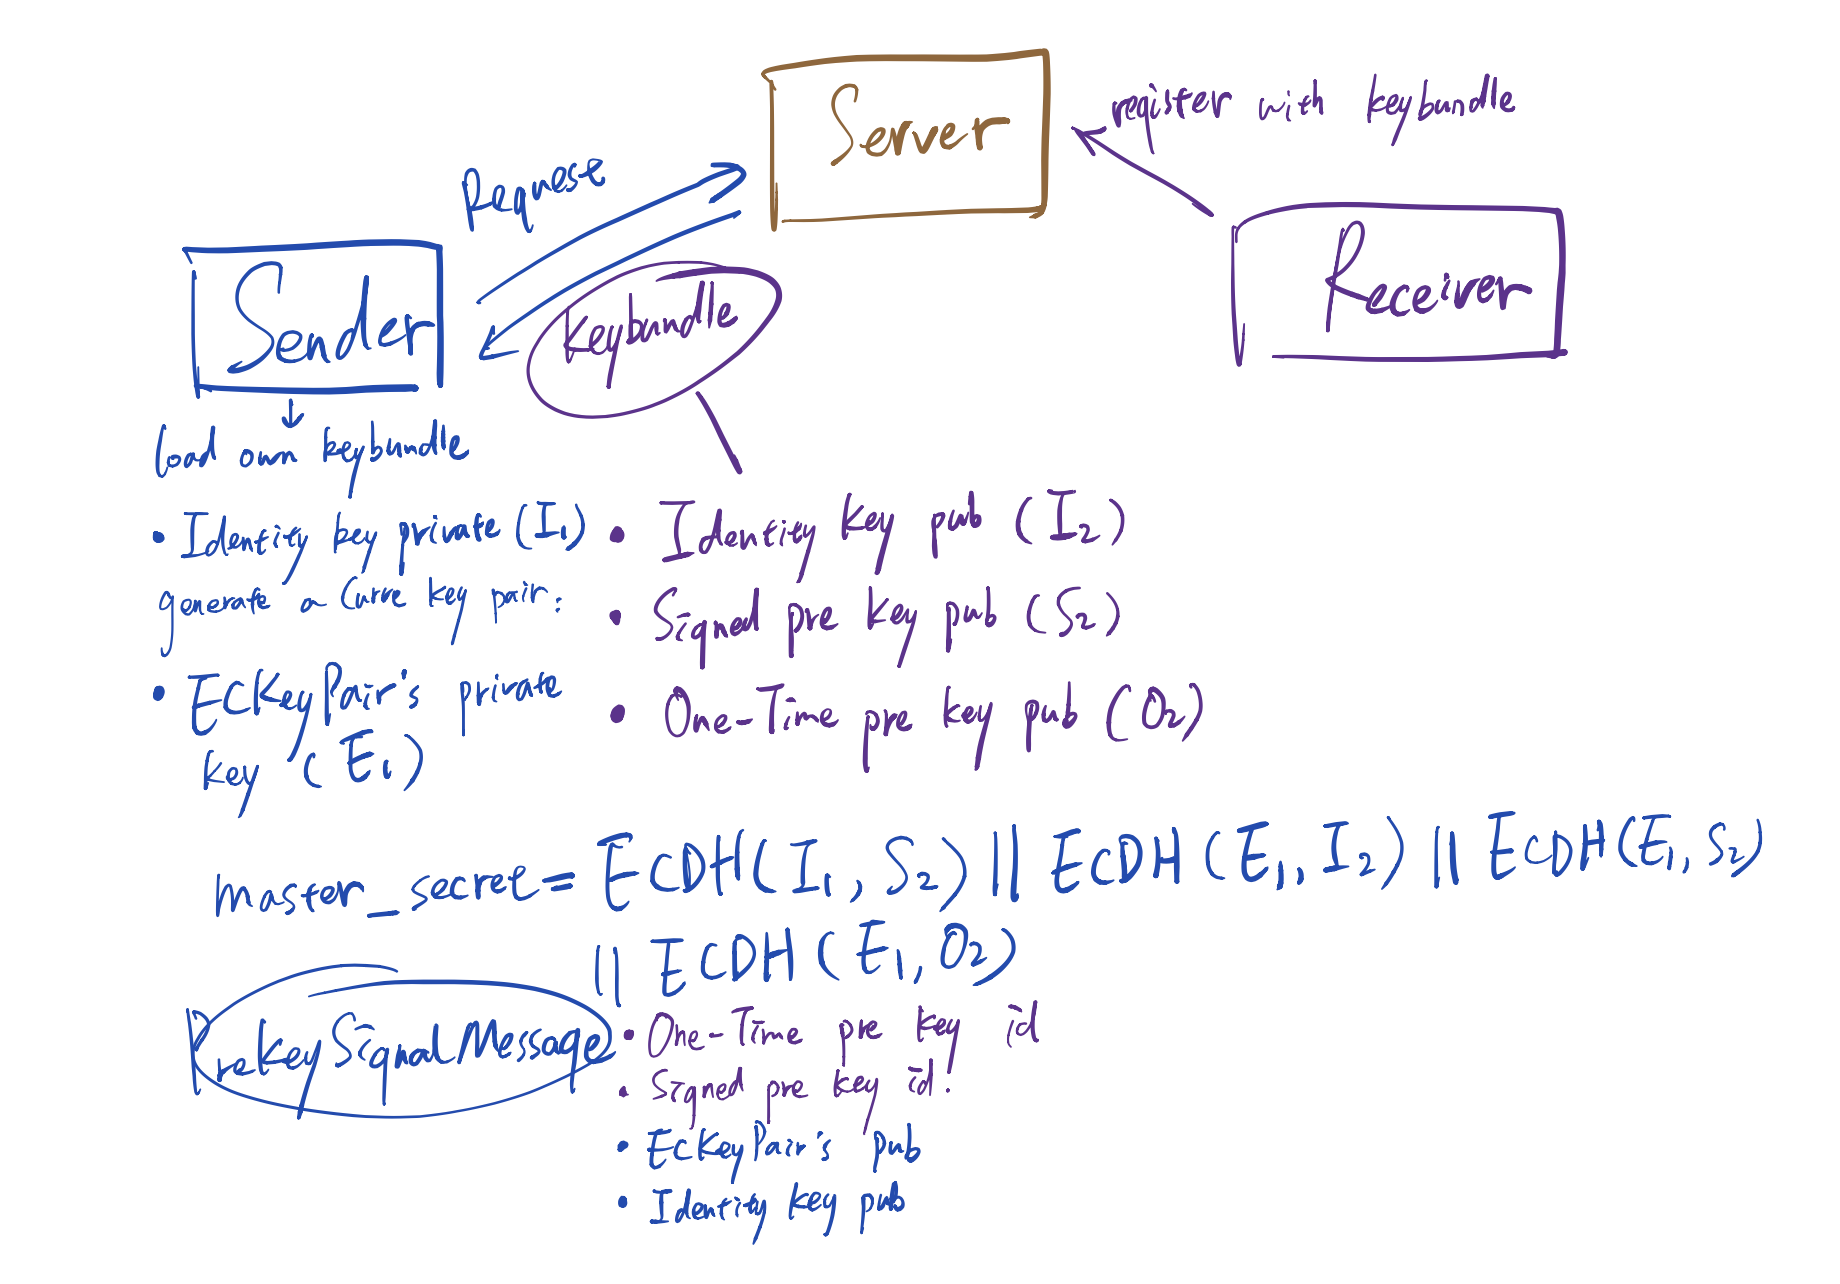
\includegraphics[scale=.5]{../3-Background/resources/X3DH.png}\\
Figure 3.1: \textit{Sender uses Extended Triple Diffie-Hellman Algorithm to initialize the pairwise chat}
\end{center}

Once the master secret is calculated, the sender needs to send his public identity key, the generated public ephemeral key and the receiver's pre keys identifier with the initial message to the receiver.

As mentioned before, the master secret obtained from X3DH is used as the first root key in root chain. Then sender needs to do the first ratchet step in Double Ratchet. The Double Ratchet is formed by DH ratchet and symmetric ratchet. The symmetric ratchet's first chain key is the output of DH ratchet, so sender needs to do the stepping in DH ratchet first. To provide the break-in recovery feature which also means future security, the DH ratchet needs an encrypted input as "salt" in the KDF algorithm. The sufficient entropy of input make the output of KDF appears random which can be used safety as the first chain key in sending or receiving chain.

The input of DH ratchet needs to have enough entropy while it also needs the confidentiality and consistency. So asymmetric encryption is a good solution to solve it. In every messaging package's header, there is a public rathcet key which is used by users to calculate the secret output via DH algorithm. In the initializing situation, receiver's public signed pre key is used as public ratchet key. The sender needs to generate a pair of ratchet keys in the meanwhile and uses the private key of it with the receiver's public signed pre key to do the DH algorithm. The output of it that provides sufficient entropy is used as the input of KDF in DH ratchet's root chain. When sending the message, the sender will send the public key of generated ratchet key pair in message header to make sure the receiver can calculate the same input of KDF in DH ratchet.

After doing the stepping in DH ratchet, root chain generated a new root chain key and a reliable output. The output is used as the first chain key in the second symmetric ratchet which means the first chain key of sending chain or receiving chain. Because the DH ratchet has already added sufficient entropy, so the output of it which is used as the input of symmetric ratchet is reliable that there is no need to add other entropy in symmetric ratchet. So the inputs of symmetric ratchet can be a constant which are usually 0x01 and 0x02. To get the message cipher key, the symmetric ratchet needs to do another stepping by using the KDF in sending chain. One stepping gets a message key which can be used to encrypt the message and once the encryption is completed, the used message key will be deleted immediately to provide the forward security. If the sender wants to send other messages in the same round, the only thing needs to do is doing the corresponding stepping in sending chain to get the right message keys. The figure 3.2 presents the whole process in detail.

\begin{center}
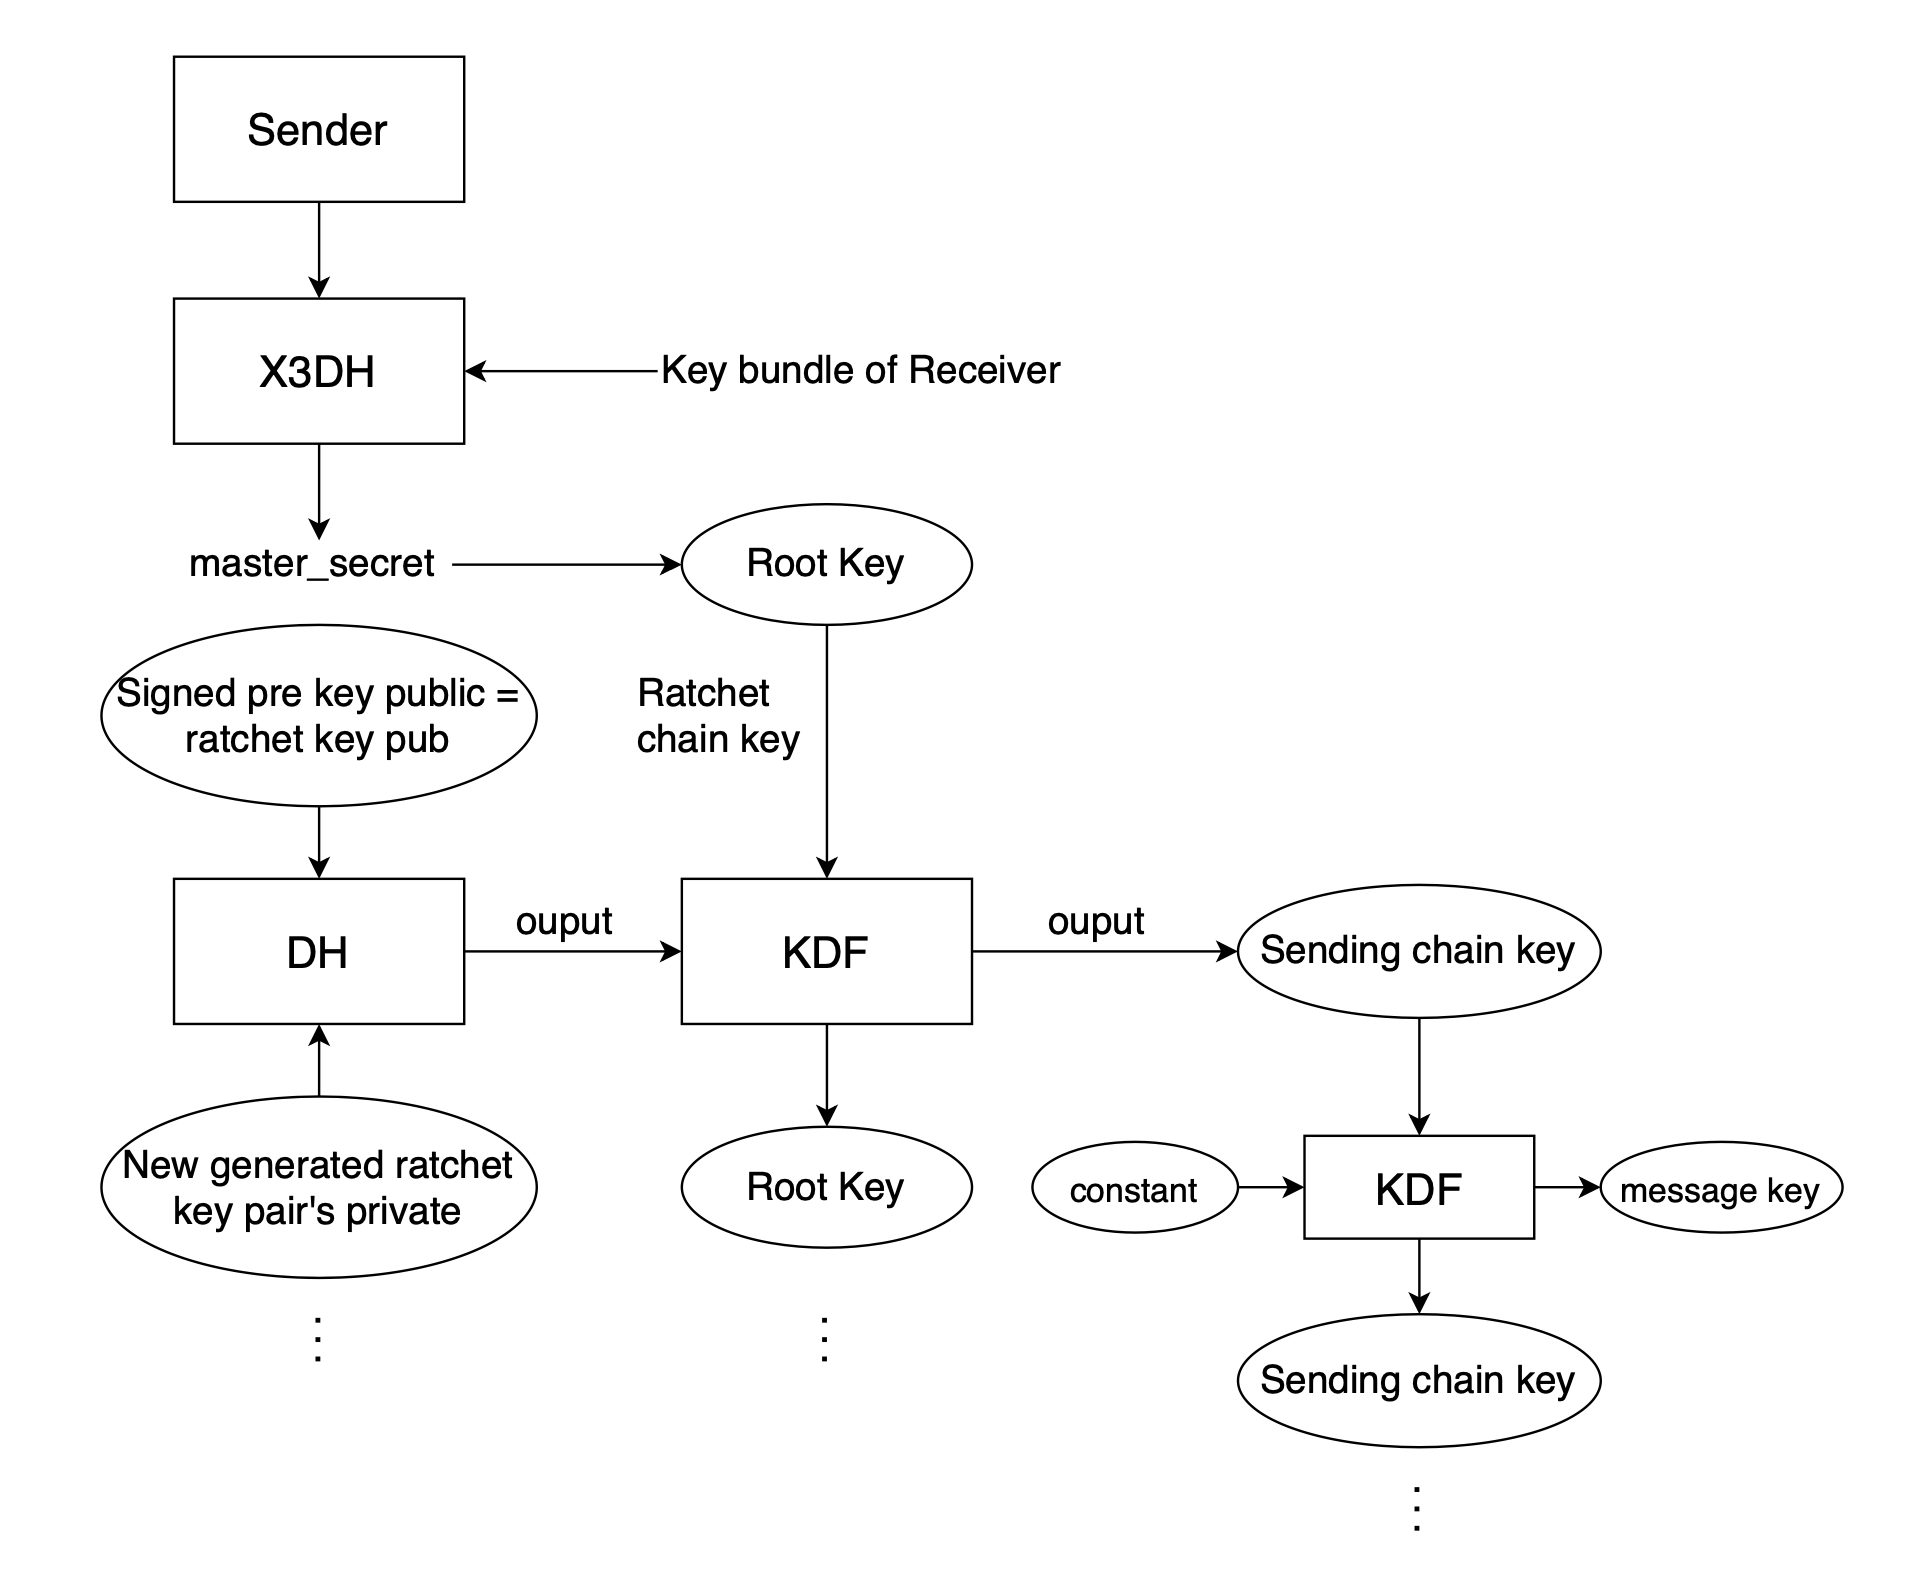
\includegraphics[scale=.5]{../3-Background/resources/DH-init.png}\\
Figure 3.2: \textit{Sender uses the Double Ratchet to encrypt the messages in the initializing situation}
\end{center}

\item Receiving Situation

In the situation that the receiver receives the encrypted messages from sender and wants to decrypt them, if the messages include the X3DH parameters, the receiver needs to calculate the root key first, or the receiver extracts the public ratchet key from message header for further decryption.

Once the public ratchet key is extracted, the receiver needs to judge it with the ratchet states first: if the public ratchet key has the corresponding receiving chain. In the situation that there is not receiving chain corresponds to the received public ratchet key, the receiver uses the old private ratchet key with the received public ratchet key to calculate an output via DH algorithm. Then the receiver uses the output as the input of KDF in DH ratchet's root chain to do a stepping. The output of DH ratchet's KDF will be used as the first chain key in symmetric ratchet's receiving chain as mentioned in initializing situation. Later, the receiver will do the right stepping in receiving chain to obtain the right message key which can be used to decrypt the received messages. Also, for the forward security, once the message key decrypted the messages, it will be deleted immediately. In the other situation that there is a corresponding receiving chain to the received public ratchet key, the receiver gets the right receiving chain and does the proper stepping in symmetric ratchet's receiving chain to get the correct message key.

The Signal Protocol is also designed to handle the out of order messages that may be caused by network delay. If the receiver receives the latter message before the former message, when the symmetric ratchet is doing the corresponding stepping, it will store the generated but never used message key with associated count. Once the former message arrives, the receiver will get the correct message key from stores to decrypt it. The figure 3.3 presents the Double Ratchet's work process in receiving situation.

\begin{center}
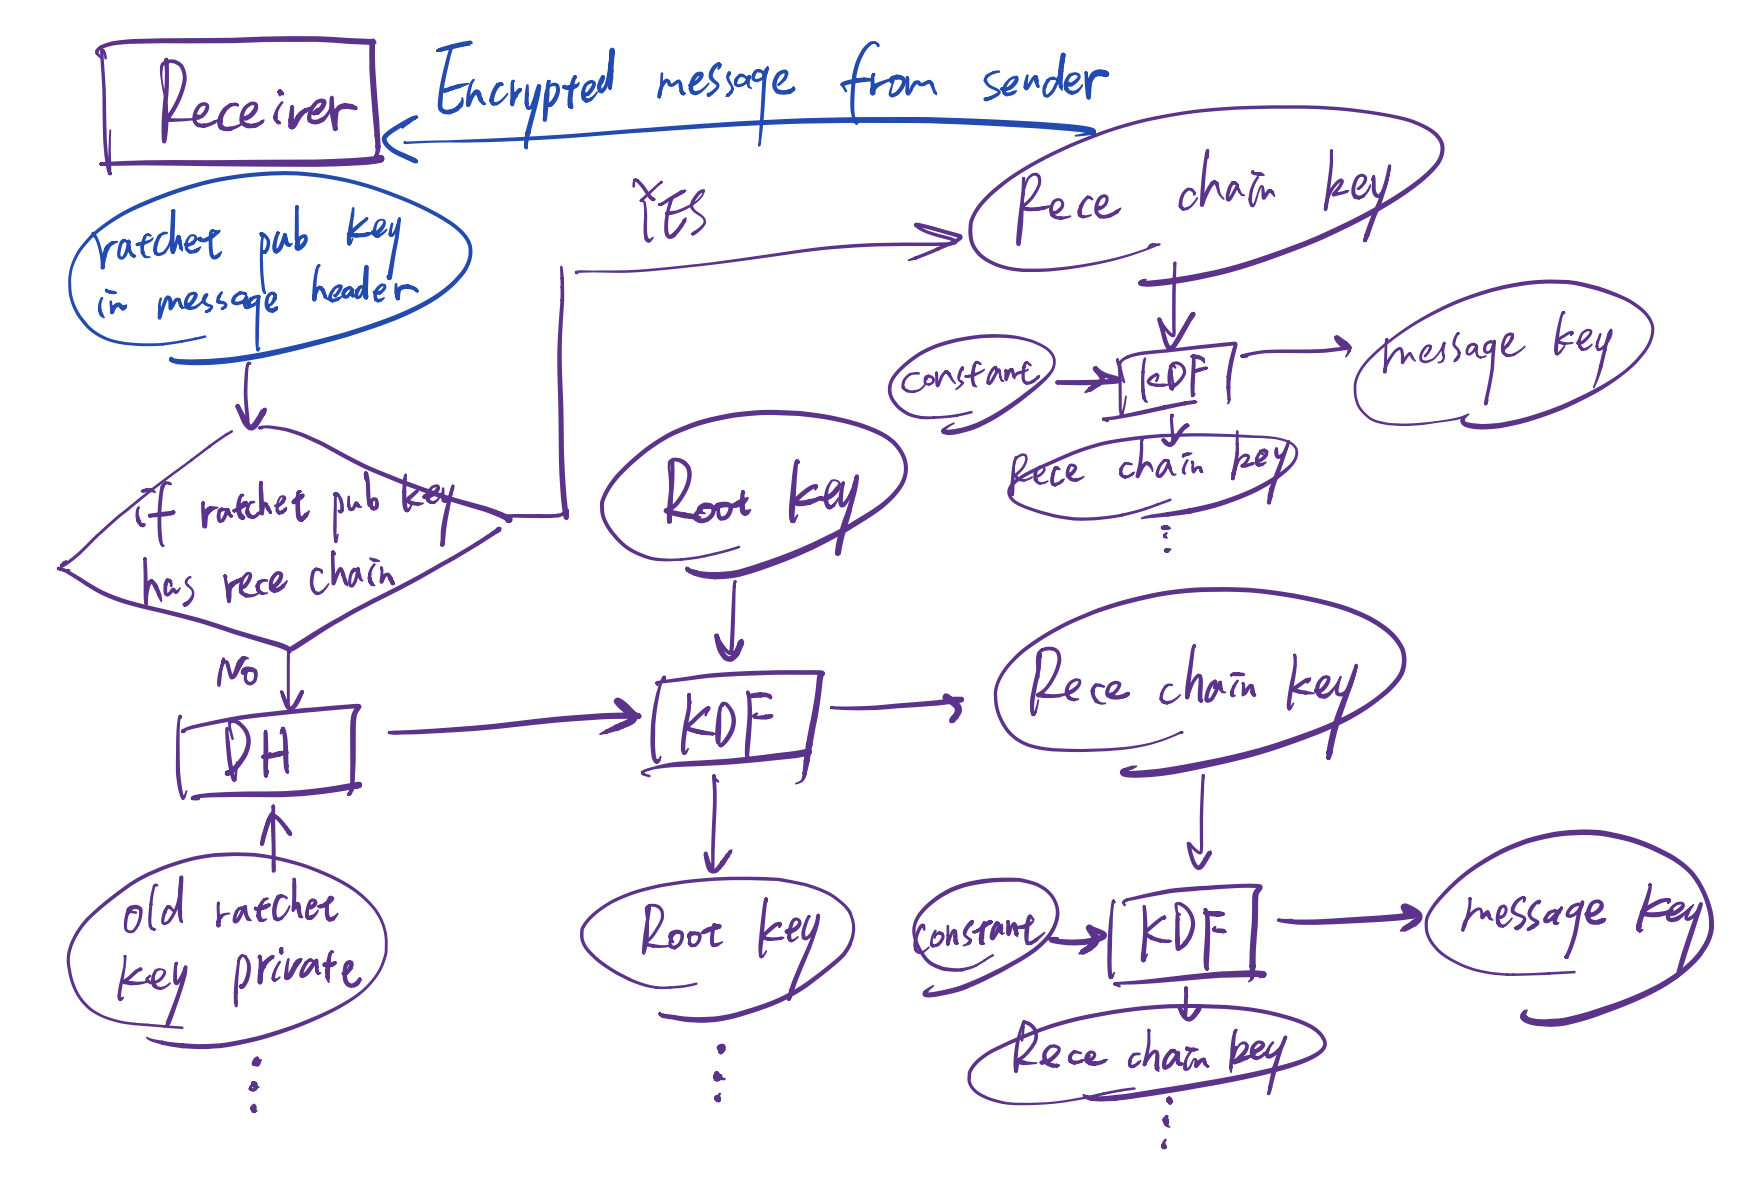
\includegraphics[scale=.5]{../3-Background/resources/DH-rece.png}\\
Figure 3.3: \textit{Receiver uses Double Ratchet to decrypt the messages}
\end{center}

\item Sending Situation

In the situation one party wants to send an encrypted message to others, it's always necessary to generate a new ratchet key pair. The user will extract the public ratchet key in latest message header first, and uses it with the private key of new generated ratchet key pair to calculate the output of DH algorithm. Then the output will be used as the input of the KDF in DH ratchet's root chain and the later steps are almost the same as mentioned in other situations before. Once the message is encrypted and prepared to be sent, the sender needs to add the public key of generated ratchet key pair in message header to make sure the receiver can do the same ratchet stepping. The figure 3.4 presents this process in detail.

\begin{center}
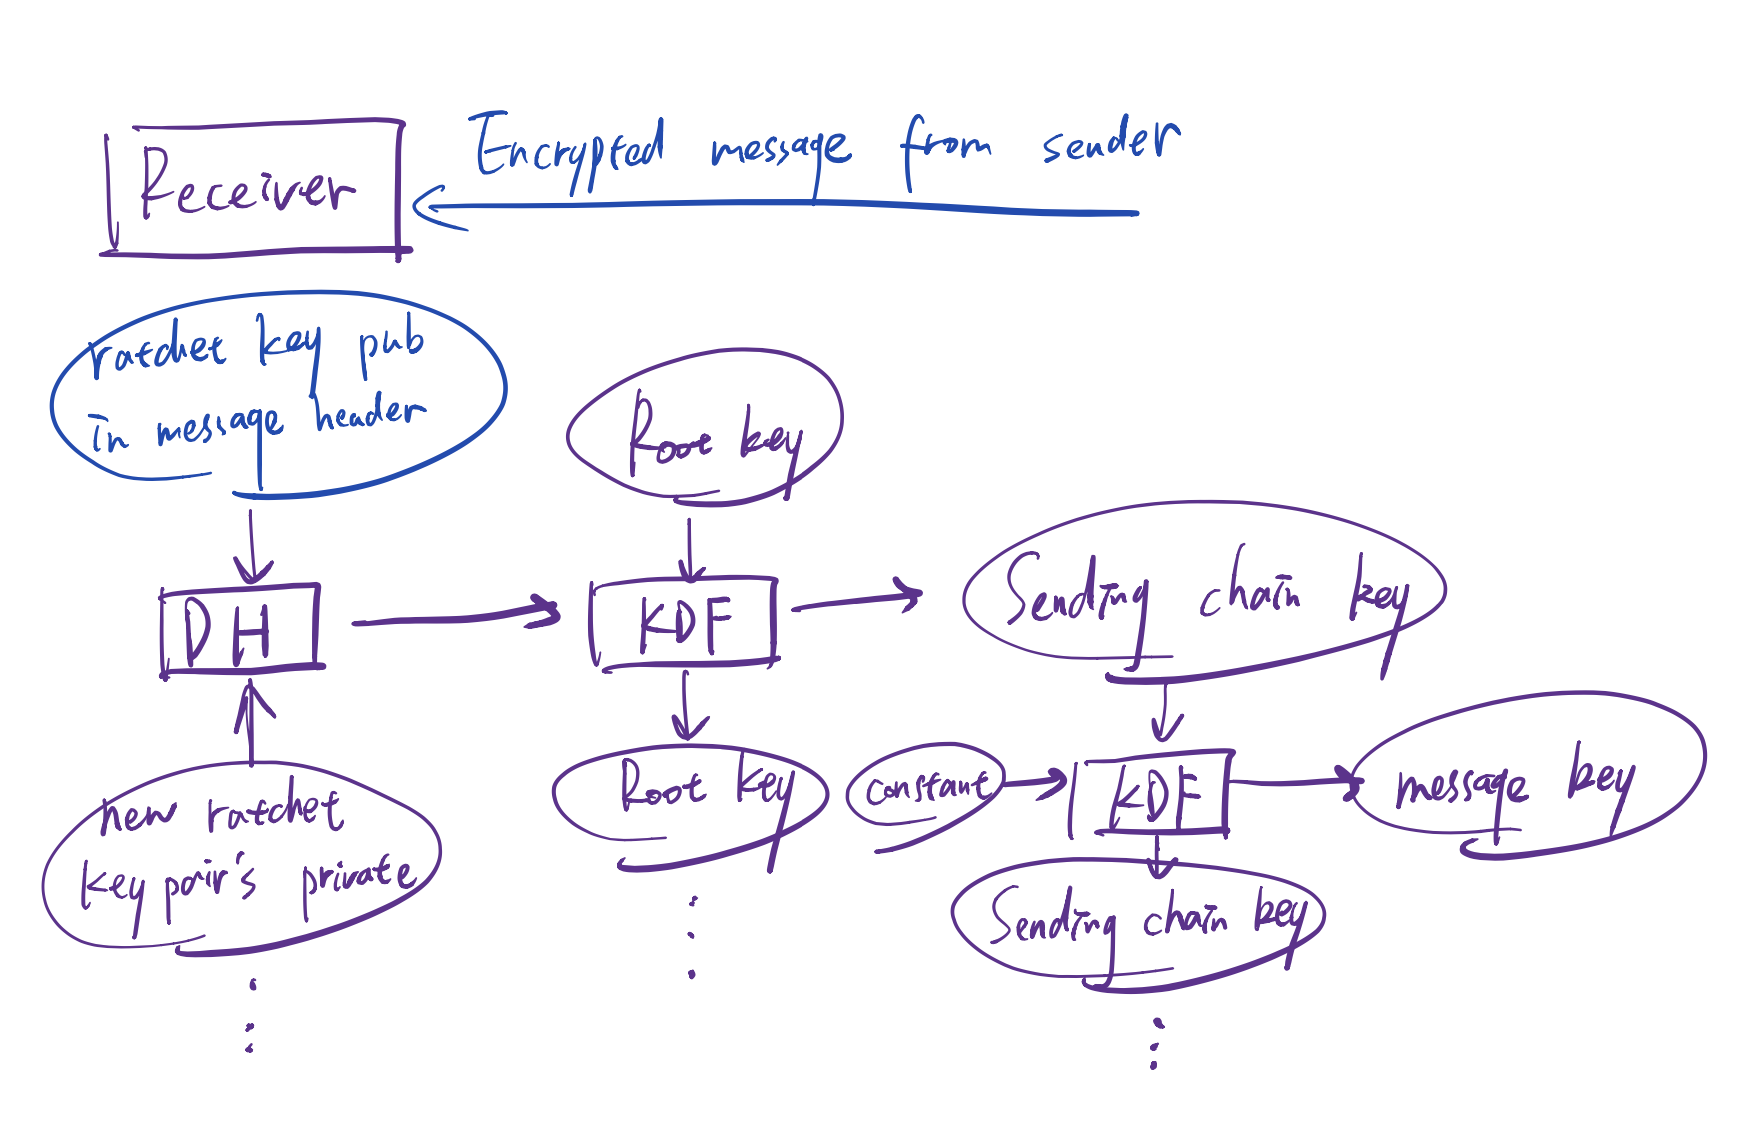
\includegraphics[scale=.5]{../3-Background/resources/DH-send.png}\\
Figure 3.4: \textit{User uses Double Ratchet to send the messages}
\end{center}

\end{enumerate}

\subsubsection{Related Work}
The Signal Protocol is a certain reliable protocol nowadays, there are several applications related to it in our life.

WhatsApp upgrades its application based on Signal Protocol in February 2017 to secure its content. Signal Protocol also has a same name chat application called Signal, which has been used by a lot of people since 2013.

 This project also borrows some strategies from WhatsApp to handle different problems in different situations, like group chat and pairwise chat's fingerprint verification function. However, since this project is developed from an existing chat system, the defect is the communication between the server and the client is special, each side has their own way to handle different type of packages. So the client cannot communicate with other Signal Compatible Server which is a regret. But the idea of Signal Protocol has been implemented in this project, it really improves the security of users' communications.

\clearpage
\section{Implementation}

\subsection{Analysis and specification}
Implementing the Signal Protocol in a chat system includes three main parts: the server, the client and the database. The server is only responsible for user login verification, messaging package forward and response to user's key bundle request etc. As the same for the database, all the user data including user identifier information and key bundles can be converted to bytes. So it's not necessary to implement the Signal Protocol on the server and database side. The focus is on the client where the Signal Protocol is used to encrypt the message data.

In the Signal system, each user has to generate a key bundle including identity key, signed pre key, pre keys and their corresponding identifiers. This key bundle is used for others to initialize the pairwise chat with the owner. To make the chat system work in the asynchronous environment, users should upload their key bundle to the server at registration. The server will convert each key in the key bundle to the bytes and insert them into the database. Once the users want to send some messages to others at the first time, they need to request the receiver's key bundle from server.

The client is asked to store the history chat messages and the Signal related states at local. Because the Signal Protocol deletes the corresponding message key immediately after encryption or decryption, storing encrypted history messages in database makes no sense. Neither the sender nor the recipient can decrypt them. To protect user's privacy at local, the system uses the symmetric encryption to encrypt all the cache files. As for the reason saving the Signal related states at local, the user should not need to initialize the pairwise chat again once the communication is established. So keeping others' key bundles and the existing chat states is essential.

In this chat system, the users are allowed to create a pairwise chat with others or have a group chat containing several users. For the purpose of users replacing or switching their devices, the system is also required to implement a multi-device system. The multi-device system allows users to switch another device and continue to have communications with others as before. Message backup function only works In the case of having both new and old devices at the same time.

\subsection{Design}
The upgraded system should keep previous functions as much as possible. Due to the limited time, the refactor of the whole system is generally not considered in this project unless the previous functions involve the terrible performance issues. Section 4.2.1 presents the main design on client side including pairwise chat, group chat and multi-device system. Section 4.2.2 presents the design on server side and section 4.2.3 is about the database structure design.
\subsubsection{Client}
The core functions on client side can be listed as pairwise chat, group chat, multi-device system and chat fingerprint verification. The following parts will introduce each function's design in detail and give the justifications for them.

\begin{enumerate}[label=(\roman*)]
\item Pairwise chat

The first function that needs alteration is the pairwise chat. The pairwise chat is relatively uncomplicated to implement. Users just need to request the receiver's key bundle from server at the first time, once the pairwise chat is established, users can send messages as simple as before. For the aim of continuous chat experience, the user should not create the pairwise chat again or lost the history chat data in the next login. The client saves the Signal storages and history chat data from cache at local. To secure the content, the client encrypt all the files with AES algorithm.

\item Group chat

The group chat is relatively complicated because of the multiple members. Assume there is a group chat containing N members. If the system adopts the program that each member creates a pairwise chat with every other one in the group, on each member's client side there will be N-1 pairwise chats. Every time the user wants to send some messages in the group, the user must do N-1 times Double Ratchet steps to encrypt different encrypted messages corresponding to the different receivers. Which means sending one message needs to do N-1 times encryptions. Besides storing all members' ratchet states is also space consuming. So this design causes large loss in time and space. The figure 4.1 presents the process of this design.

\begin{center}
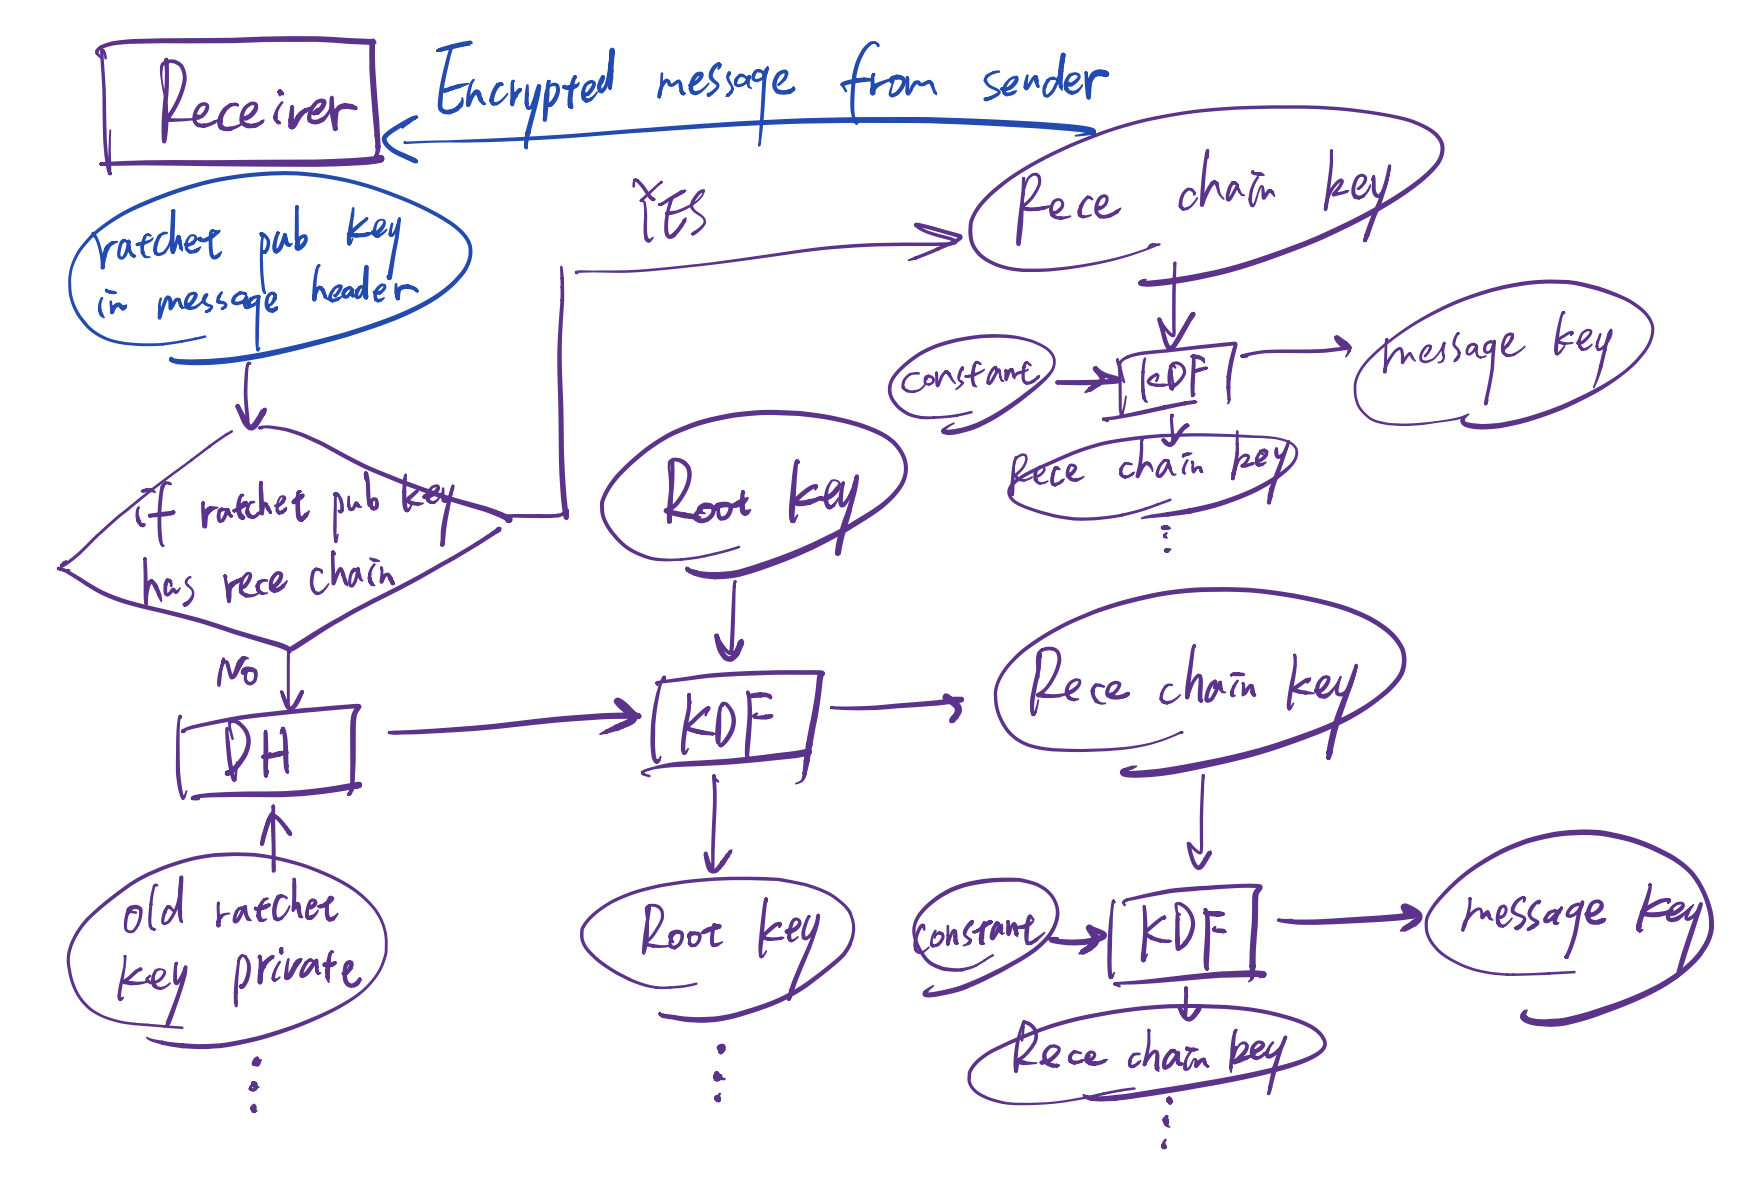
\includegraphics[scale=.5]{../3-Background/resources/DH-rece.png}\\
Figure 4.1: \textit{Implementing group chat by creating the pairwise chats between each other}
\end{center}

Fortunately, WhatsApp and Signal have already given the solution. Because of the high security feature of Signal Protocol in pairwise chat, members can exchange their chain keys via pairwise way. When the group chat is initializing, each member needs to generate a sending chain key as the second ratchet in Double Ratchet. Then they should use the pairwise chat to exchange their sending chain key with every other one in the group. After initialization, on each member's side there are only N-1 sending chain of others and one own sending chain. Every time the user wants to send some messages in the group, the user only needs to do a stepping on his own sending chain and get the correct message key for encryption which means one message only needs one encryption. For the receivers, they just need to find the correct sending chain corresponding to the sender and do the correct stepping to get the message key for decryption. This design is much better in time and space cost then the former. The figure 4.2 is the schematic diagram of it.

\begin{center}
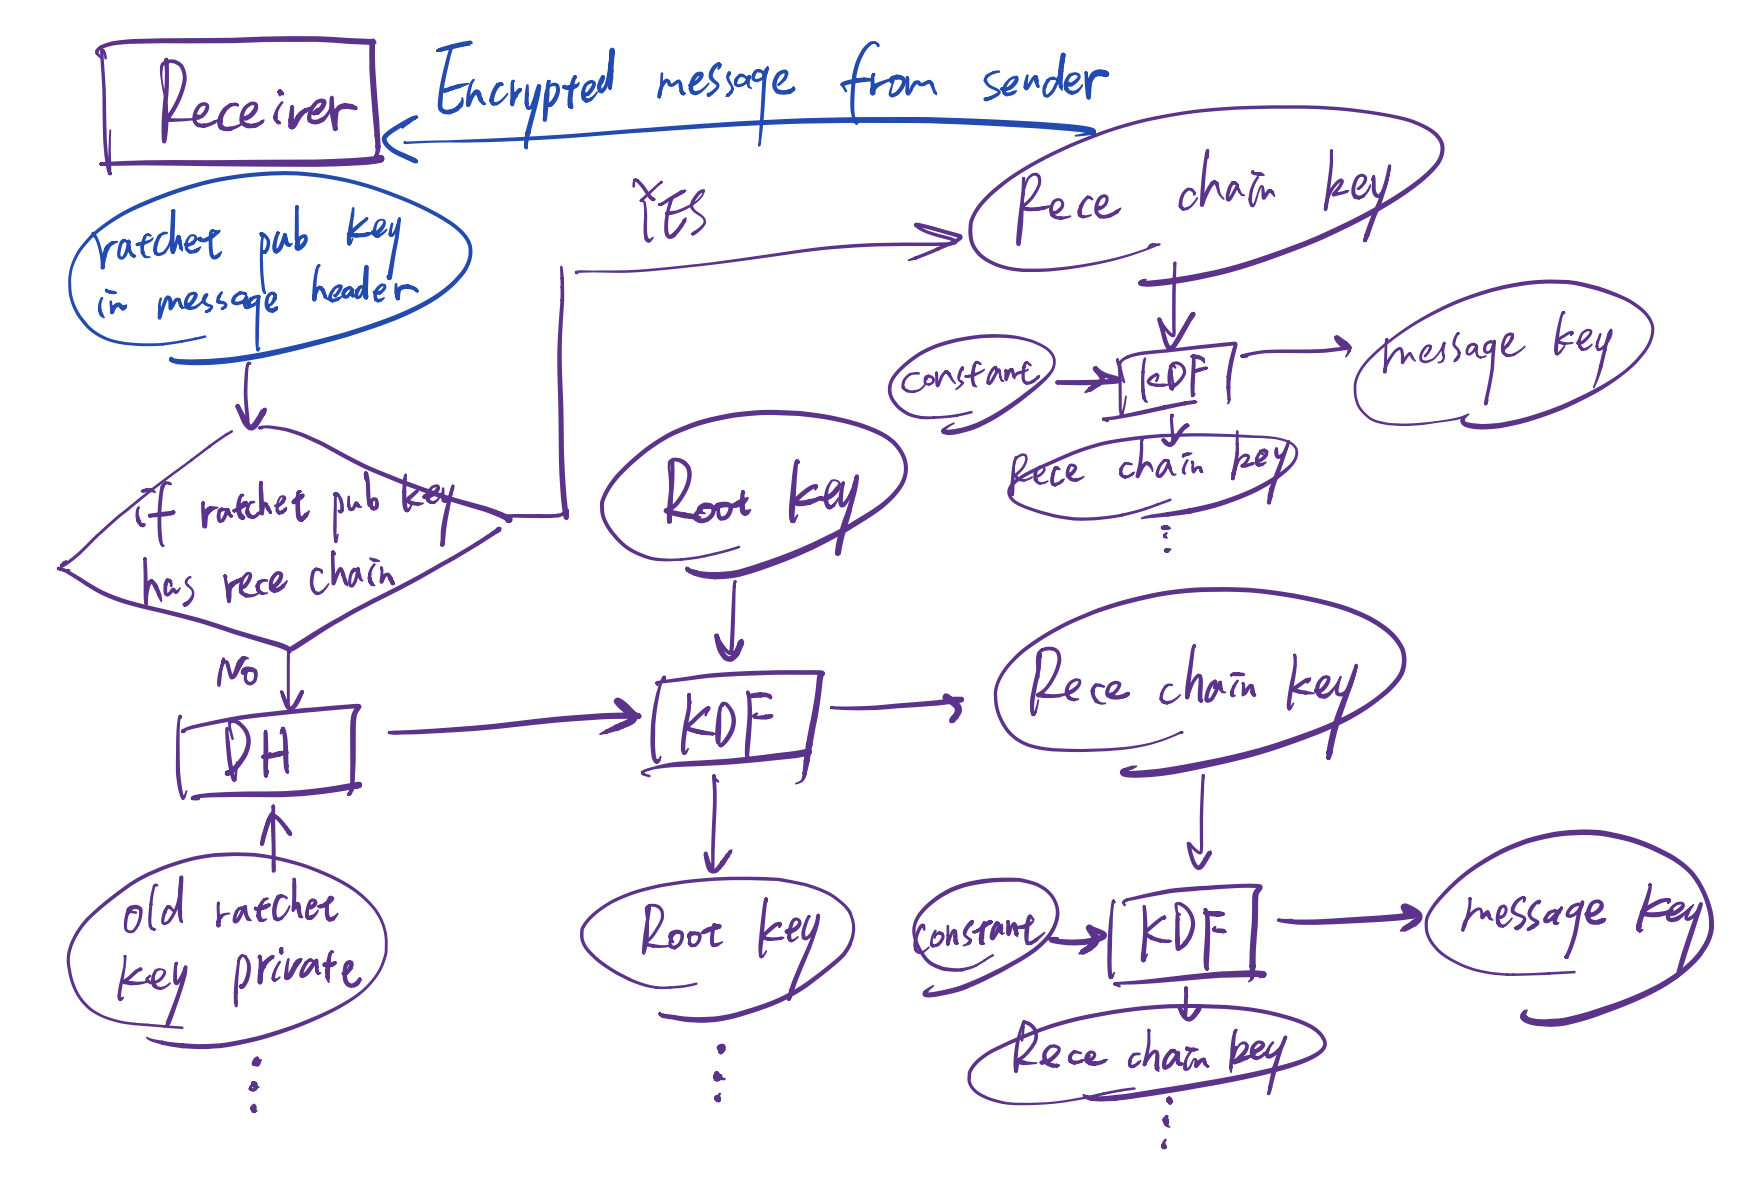
\includegraphics[scale=.5]{../3-Background/resources/DH-rece.png}\\
Figure 4.2: \textit{Implementing group chat by creating the pairwise chats between each other}
\end{center}

\item Multi-device system

Switching device is an important function in a chat system. It allows users to get continuous using experience while changing their device. Because the Signal Protocol requires each account generates the unique key bundle for communication and the confidentiality of the private keys is the precondition of the chat's security. So to some extent, Signal Protocol is device-oriented. User's each device needs to generate a unique key bundle as a new account. In this system, there should be a new customize class User containing the username and deviceId fields, which means one user can have several accounts with same username but different deviceId. The figure 4.3 shows the user information structure in multi-device system.

\begin{center}
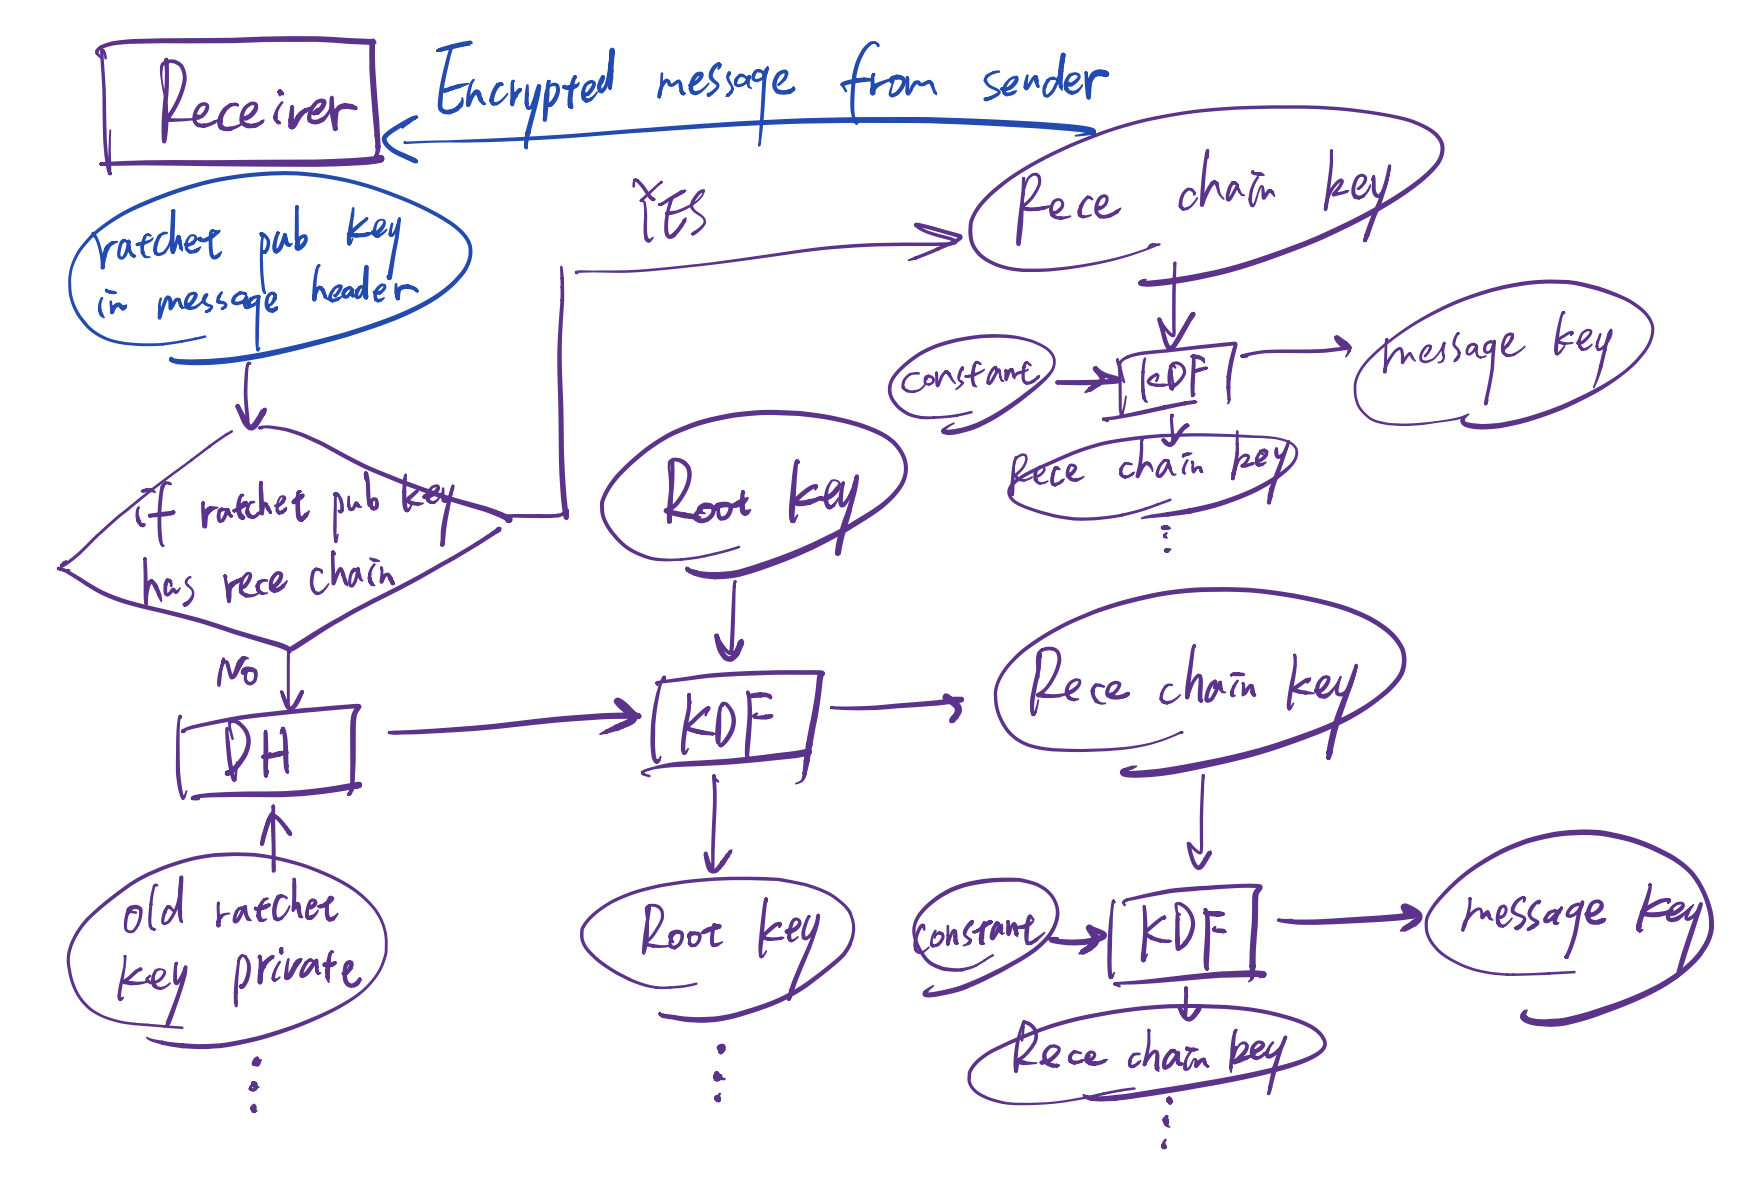
\includegraphics[scale=.5]{../3-Background/resources/DH-rece.png}\\
Figure 4.3: \textit{The user information structure in multi-device system}
\end{center}

When the user switch the device at the first time, it's necessary to register a new account with the same username and password but different deviceId. The requirement of the same password is to prevent adversaries' malicious registration. In the meanwhile, the new account generates a new key bundle and upload it to the server for further communication. The login function is also asked to change: the user's login information should include username, password and deviceId for the server to judge if this account is registered.

Once the user successes to switch the device, the old pairwise chats and group chats related to him on other's client side are still not updated. The messages from others are forwarded to the old device so that the user cannot receive the corresponding messages from others. To solve this problem, the system decides to inform all users when the user is switching device. Users will judge if there is any chat related to the switching user and update the switching user's information and key bundle from server if yes.

To avoid other users to send messages to the old account, the client will be inoperable while updating the switching user's information and key bundle. Once the client completed the update, users can send messages as before.

The update of switching user's information can be considered in two situations. In the pairwise situation, if there is corresponding session related to the switching user in Signal's session store, users need to request the switching user's key bundle of new account from server and update the chat session's member information. The alteration in group chat situation is relatively complicated. First users need to find the related group chats that contain the switching user in group members. Then they are supposed to generate a new sender key for later group communication. The reason for this operation is to guarantee the future security of group chat, because the switching user's old device maybe lost and exploited by the adversary to get later communication data if not changing each member's sender key. After generated the new sender key, users need to distribute it to every other one in the group chat as initialization. Users may do not initialize the pairwise chat with the switching user's new device, so before distributing the sender key, they need to initialize the pairwise chat to create a secure connection with the new device. Then the encrypted sender key can be delivered to the switching user's new device for further group chat. On switching user side, the user will judge if there is corresponding own sender key related to this group at the moment of receiving other's sender key. And the user will generate and distribute the new sender key if no. After all these operations, the group chat can work with the switching user's new device as before.

As for the consideration of message backup, the multi-device system adds a field variable named active while login. The user could only have one active account at the same time. If the account which is logging in was not active previously but would be active now, the multi-device system would update user's active account information to complete the device switch operation. When the account which is logging in was inactive previously and would not be activated now, the account could send the backup messages to the active account of the user. The figure 4.4 has an overview about the login handle in multi-device system.

\begin{center}
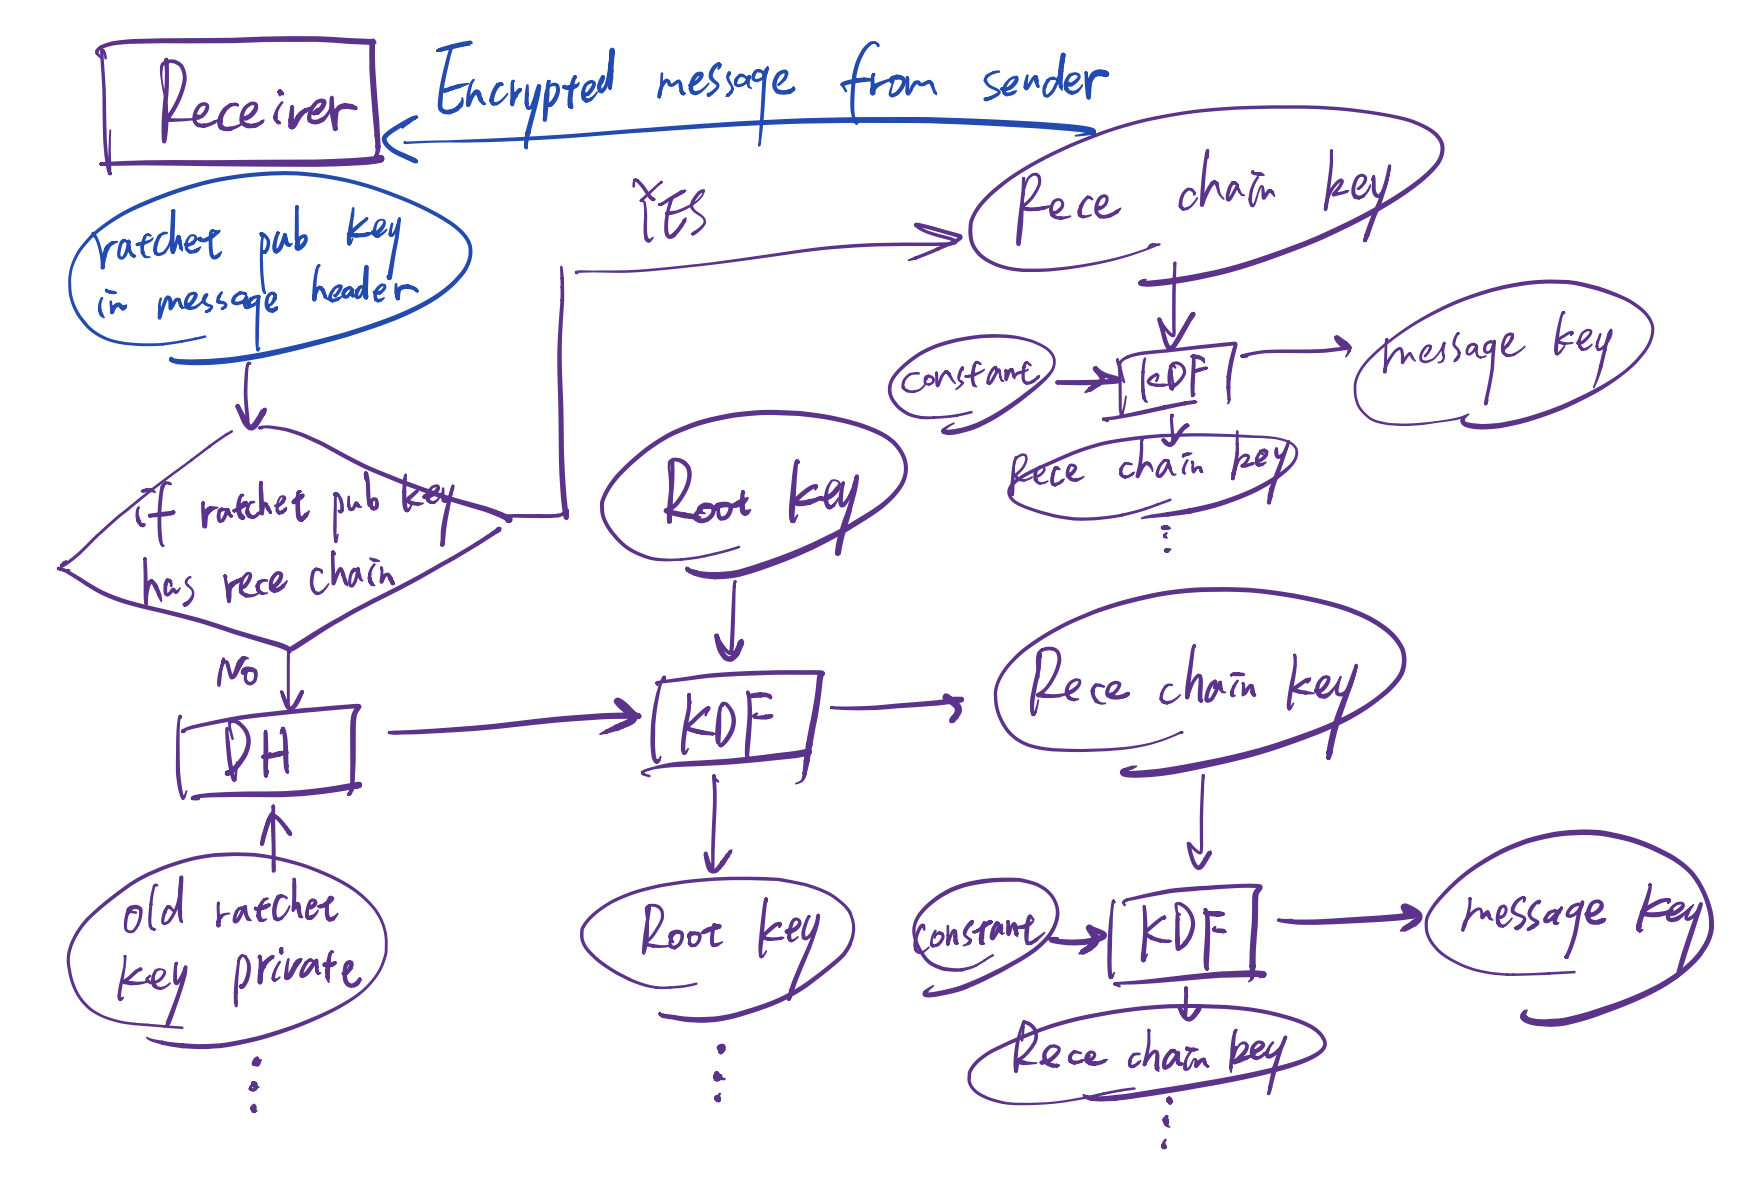
\includegraphics[scale=.5]{../3-Background/resources/DH-rece.png}\\
Figure 4.4: \textit{The login handle in multi-device system}
\end{center}

\item Chat fingerprint verification

The guarantee of Signal Protocol's security is that the both parties are indeed themselves. The secure pairwise chat can be monitored via MIMA (Man In The Middle Attack). As a simple example, the server serves as the adversary and wants to monitor the communication content between two users called Alice and Bob.

At the initializing time, Alice requests Bob's key bundle from server. However the server responses its own key bundle to Alice. Once the Alice completed the ratchet steps and encrypted messages, the members in this pairwise chat is Alice and server in fact. Then the server uses the Signal Protocol to decrypt the encrypted messages from Alice and establishes a secure pairwise chat with Bob using its own and Bob's key bundles. After that, the server encrypts the plain text from Alice again in the chat containing Bob and delivers it to the Bob. Until now, the server has two secure connections with Alice and Bob respectively and can decrypt the messages between them easily without their knowledge.

The key to solve this problem is how to ensure the two parties are the same in their perspective. In both parties' perspective, this pairwise chat's members should be Alice and Bob. However, on Alice's side the members of this pairwise chat are Alice and the server, on Bob's side the members of it are Bob and the server in fact. So comparing the two chats' identifiers is a good solution to check whether they are hijacked. The pairwise chat's fingerprint is generated using two parties' public identity keys and can be presented by a series of bytes. The two parties can compare own chat's fingerprint with the other's fingerprint via other communication ways but not the same pairwise chat. Because if they still use the previous pairwise chat to exchange their fingerprints, the server can replace the content of fingerprint for confusion. Once the users find they are monitored by adversary in pairwise chat, it's essential to update sender keys in all related group chats too. To reassure users that the server is not monitoring their communications, Signal Protocol is not used on server side in this system, but this function is still useful to prevent MIMA from adversary.
\end{enumerate}
\subsubsection{Server}
The server's duty in this system is responding to users' requests and forwarding users' messaging packages. 

In login and sign up functions, the server needs not only verify user's username and password, but also judge if the deviceId is registered or existing due to the alteration of User class.

The server is also required to respond to user's key bundle requests. Once received the key bundle requests, the server will inquire the key bundles from database corresponds to the userId.

In order to match Signal Protocol's asynchronous feature, the server is supposed to be designed to work in asynchronous. For example, Alice wants to send some encrypted messages to Bob who is offline currently. The server cannot find Bob in current online users list and stores the messages in cache. Once the Bob logins at some time, the server will load all related messages and send them to Bob as soon as possible. After that, the server will delete sent messages in cache to release the memory. This caching strategy is also applied to sender key distribution, switch inform and backup messages etc.

In the logout function, since the client stores history messages at local, there is no need for the server to handle it any more. The server's only duty in this function is informing other users which one is logging out.
\subsubsection{Database}
There are only two tables in the database, the Users table and KeyBundles table. To be compatible with the multi-device system, the User table is required to add a new field deviceId. The KeyBundles table contains the key bundles associated with corresponding users. Since the history chat data is not saved in database any more, the ChatData and Session table can be dropped. Figure 4.5 presents the table structure of Users and KeyBundles tables.

\begin{center}
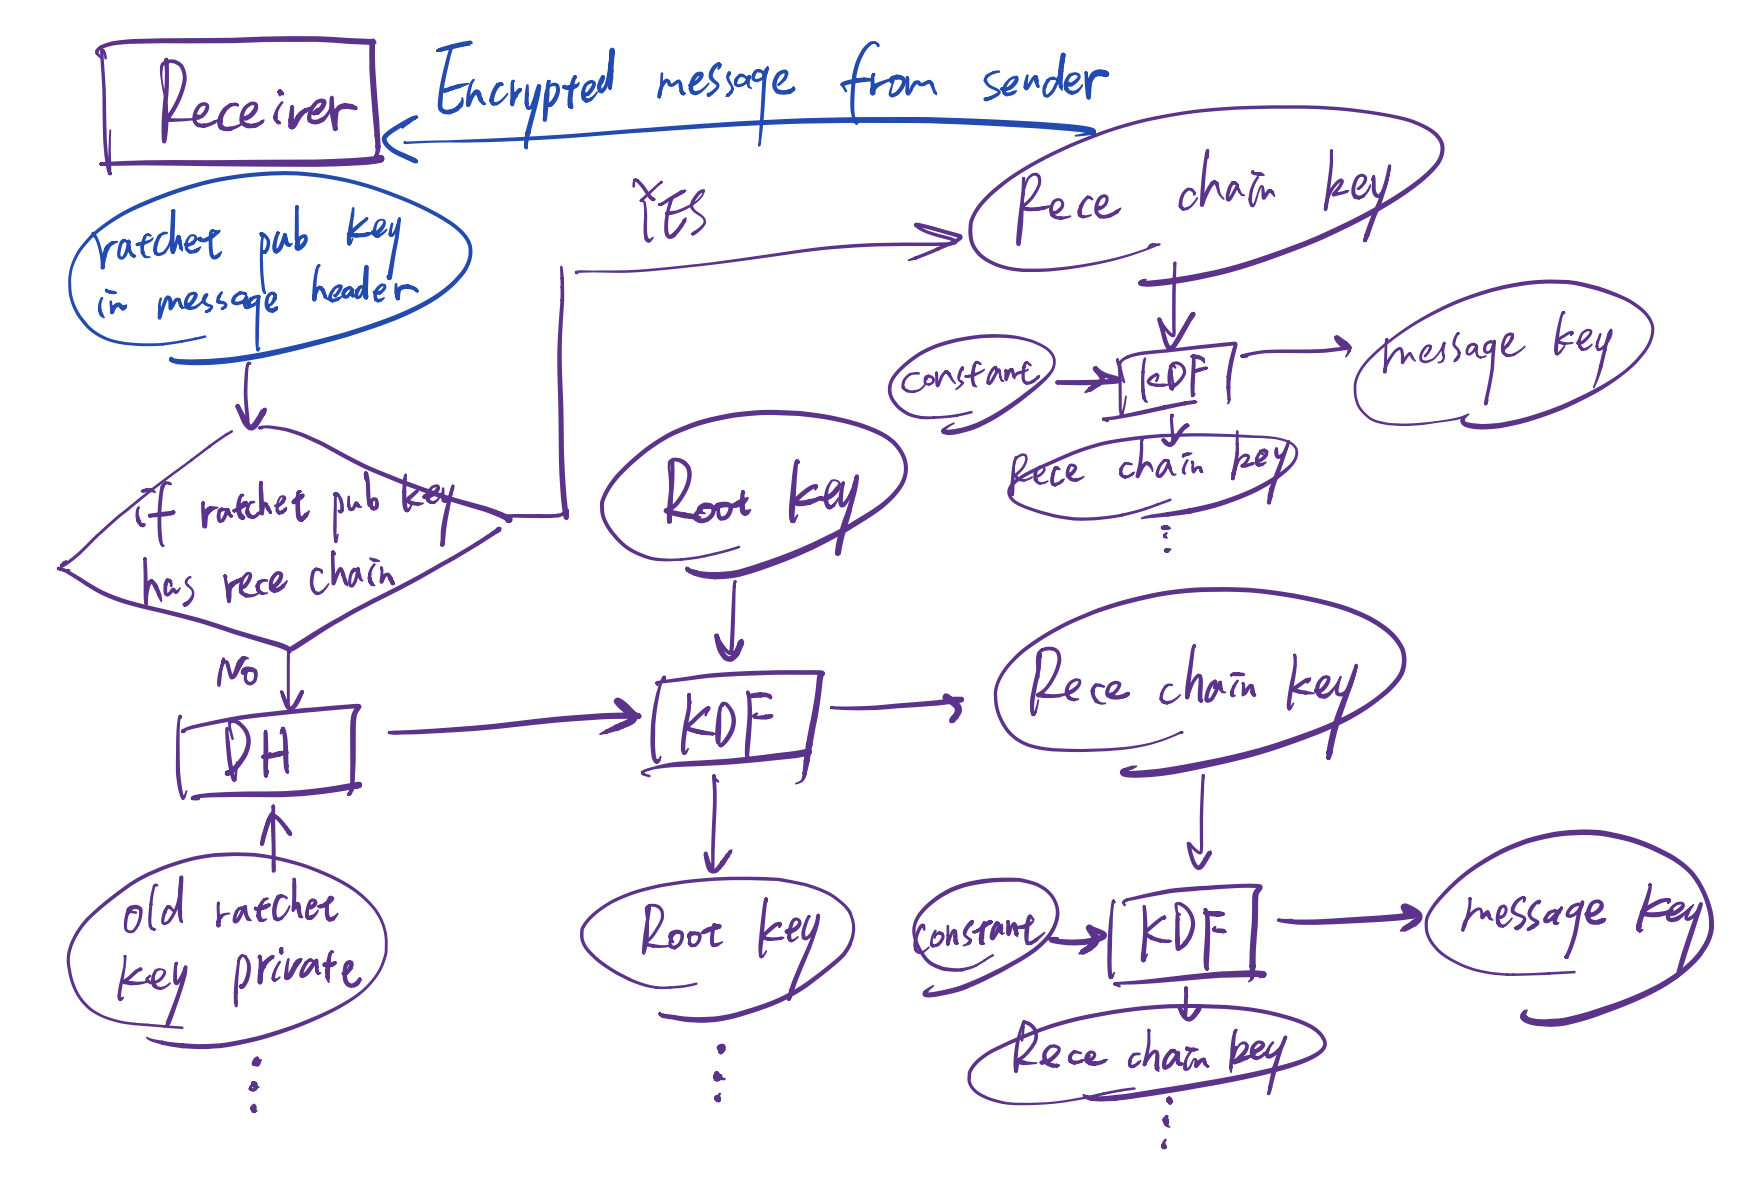
\includegraphics[scale=.5]{../3-Background/resources/DH-rece.png}\\
Figure 4.5: \textit{The structure of Users and KeyBundles tables}
\end{center}

\subsection{Implementation and testing}
The concrete implementation in this project can be divided into three main parts including the client, server and database. The first few sections will describe the implementation details and the justifications on corresponding side. The last section introduces the testing strategy and presents some testing examples of the whole system.
\subsubsection{Implementation in Client}
The main work in the client includes the implementation of Signal stores, development of pairwise chat and group chat, updating session information while devices switching and the verification of pairwise chat fingerprint. All the Signal related behaviours are put in the EncryptedClient and EncryptionHandler class such as the creation or load of Signal stores, encrypted chat initialization and message encryption.

\begin{enumerate}[label=(\roman*)]
\item Implementation of Signal stores

The libsignal-protocol-java lib provides several Signal store interfaces for developers to implement. There are all kinds of ways to implement them. These stores keep the Signal related states including identityKeyStore, signedPreKeyStore, preKeyStore, sessionStore and senderKeyStore.

Each store maintains other users' certain public keys. For example, identityKeyStore maintains other users' identity keys, signedPreKeyStore maintains others' signed pre keys. The data structure storing related keys that the implementing class used is HashMap. Map is a suitable data structure to save the KV pair. In these Signal stores, the key and value in the KV pair is the account and their keys respectively. HashMap is an efficient implementation of Map, since there is no need to order keys in Signal stores, using HashMap can improve the accessed speed.

Once determined the data structure of storage, the implementation of constructor, setters and getters is more easier. After constructing the Signal stores, the user needs to add their own signed pre key and pre keys in SignedPreKeyStore and preKeyStore respectively. Otherwise the user cannot recognize their own keys in further session's initialization.

Besides, developer can add some other functions in the implementing stores such as serializing the keys in the storage and judging whether there is any related session in sessionStore. All the functions related to the Signal stores can be implemented in them to keep the code in Object-Oriented style.

\item Development of pairwise chat and group chat

The core functions during the chat are initializing the chat and encrypting or decrypting the messages.

During pairwise chat initialization, once received the key bundle from the server, the client will invoke the pre-packaged functions in Signal lib to create a corresponding session. Then a sessionCipher that used for further encryption and decryption can be generated via Signal lib's function. The same situation in group chat is relatively complicated. When the user wants to create a new group chat, the client will invoke the initGroupChat function. In this function, the client will generate a new sender key for this group chat and judge if there is anyone who has not created a pairwise chat before. After establishing secure communication with all other members, the client will start to invoke the distributeSenderKey function to encrypt and distribute its own sender key to others. In the meanwhile, the client is also supposed to handle others' sender keys -- storing them in the senderKeyStore's HashMap for further decryption. Then a pre-packaged class from Signal lib called groupCipher can be generated for further encryption and decryption. JavaFx will generate a waiting alert to make the client inoperable during the initializing process until the client's own sender key distributed. Because if the group messages delivered before the sender key, the receiver cannot decrypt them with the correct sender key.

While communication, the client can invoke sessionCipher's encrypt or decrypt function from Signal lib to secure the chat content. The encrypt function is wrapped in EncryptionHandler class for both pairwise and group chat invocation. The output of it is serialized to bytes for the transmission convenience.

\item Session update while devices switching

For the continuity of the chat, the client is required to update related session members' information while the user is switching device. Once the client received the switching inform from the server, it will check whether there is any related pairwise chat or group chat immediately. Judging the related chat session in history chat data is not reliable, because the pairwise connection may be established while the group chat initialization but there is no chat session record in history data. The wiser choice is using the sessionCipher and senderKey to judge if there is any related session needs to be updated.

The client will request the user's key bundle of new device to reinitialize the pairwise chat and generate a new sender key which will be distributed to others to reinitialize the group chat.

During these processes, the client invokes javaFx's function to generate a waiting alert to make the application inoperable. The reason for it is to avoid users to lost the messages before the switching completed.

\item Pairwise chat fingerprint verification

To help the users to figure out whether they are monitored while communicating, the client has the function getFingerprint according to the pairwise chat parties. The function constructs a pre-packaged class from Signal lib called NumericFingerprintGenerator and invokes the createFor function to generate the fingerprint of pairwise chat. There is a button on the head of the chat, once the user clicked it, the client will use javaFx to generate a information alert which shows the fingerprint string for user's comparison.
\end{enumerate}

\subsubsection{Implementation in Server}
The functions that are required to be implemented can be listed as three parts: response to users' requests, storage of undeliverable messages and user identify verification.

\begin{enumerate}[label=(\roman*)]
\item Response to users' requests

To construct a Signal compatible server, the server is supposed to have the ability responding the users' Signal related requests. For example, the users will request other's key bundle while initializing the pairwise chat and send their sender key to the group members.

This system uses socket programming to implement the communication between the server and the client. There is a common class on both server and client side called ConnectionData representing the package data during connection. This class must be same on both sides or it will be serialized to the bytes that the other side cannot deserialize. Both client and server process the data reception by an independent thread. Once the party received a connectionData, it will deserialize the connectionData first and then do some operations corresponds to the type of data. The figure 4.6 presents the structure of ConnectionData and the process of communication between the server and client.

\begin{center}
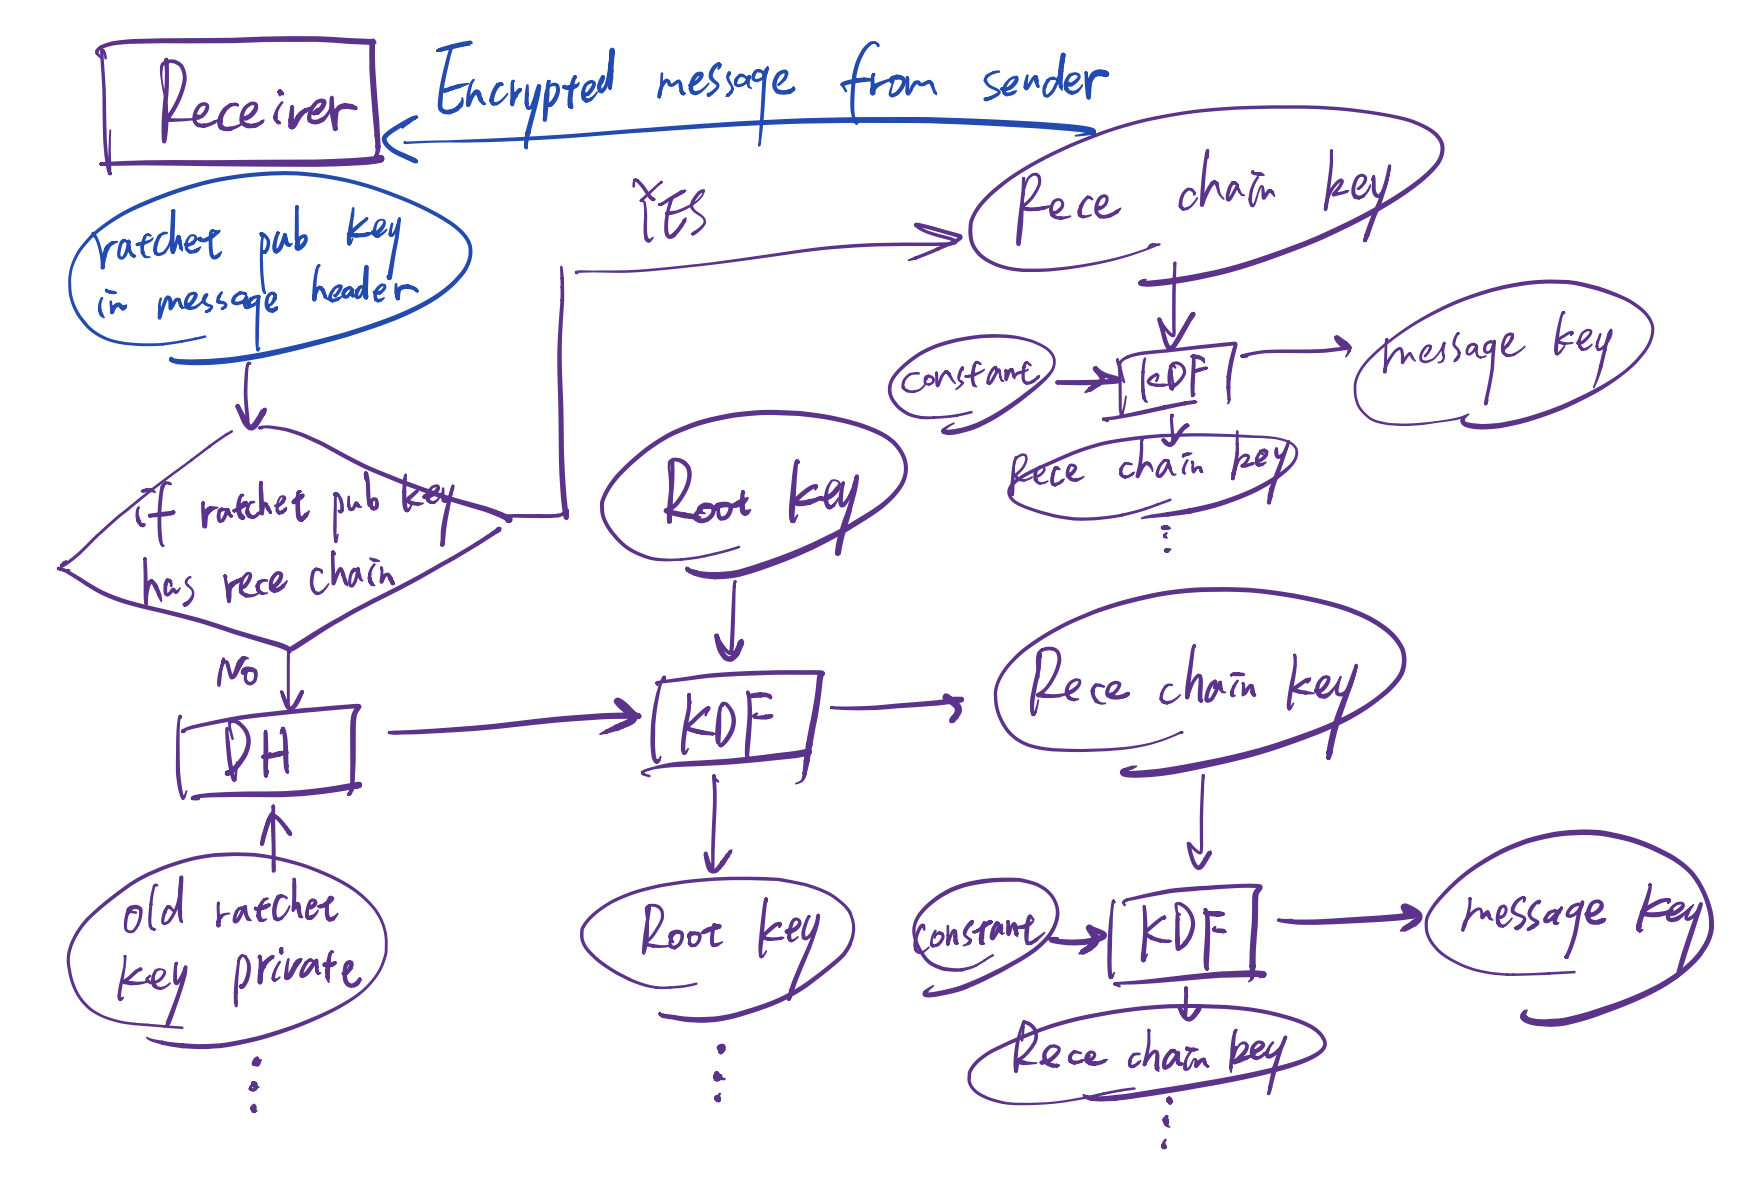
\includegraphics[scale=.5]{../3-Background/resources/DH-rece.png}\\
Figure 4.6: \textit{The process of communication between the server and client}
\end{center}

The ability of responding the user's key bundle request is essential in a Signal system. The server adds a new filed variable in connectionData named keyBundle to represent the key bundle payload and defines the type of this kind of connectionData. While processing the key bundle request, the server would inquire the certain key bundle from the database by associated userId. If the key bundle is not found according to the given userId, the server would throw an IllegalArgumentException for alerting.

Other functions of responding to user's requests are almost the same as the key bundle request function. Because the I/O architecture in both server and client is synchronous, sometimes the communication between the server and client is quite complicated for development. For an instance, while reinitializing the group chat due to the device switching, there may be several situations needed to be handled, the following steps are required to be written repeatedly in every situation branch. In some processing scenes, the server uses package combination strategy to solve this problem. For example, the server would combine all the key bundles together in one response when the user requests several users' key bundles at one time.

\item Storage of undeliverable messages

Storing the undeliverable messages in server's cache is an essential solution for asynchronous messaging environment. Sometimes the messaging receiver may be offline so that the server cannot deliver the messages correctly. In this situation, the server would store the messages until the receiver is online again, then send and delete them.

For the implementation of this function, the server maintains several storage including depositPairwiseData, depositSenderKeyData, depositGroupData, depositSwitchData and backUpMessages. The data structure that these storages used is HashMap which can store the KV pair efficiently. In the first four storages, each user account corresponds to an ArrayList containing the related connectionDatas. In the last backUpMessages, each user account corresponds to another HashMap containing the history backup.

Every time the server processing the package forward, the server would try to get the outputStream according to the user account first. If there is no related outputStream, the server would put the message in the corresponding storage's HashMap with related user account. Then while every user's login, the server would traverse all the storages to get the associated messages and deliver them to the user. In the getting deposit data functions, the deletion operation at the end is essential or the user would get the same message again in further login.

\item User identify verification

After implemented the multi-device system, the user identify verification needs alteration too. The information of user is expanded by a new filed variable: deviceId. In the initial design, a user could have several accounts with the same username and password but different deviceId. In the meanwhile, a user could only have one active account at the same time. The active account is the account that others' messages would be forwarded to. While switching accounts, the user could choose to activate the account or not. If the user activates the account which means the user switches the account normally, the server would inform all the others to update the session information. If not, the user can login to that account without activation for message backup.

So the verification of user identify should consider the username, password, deviceId and activation. In the login situation, the server would inquire the records of given username, password and deviceId. If the result set is empty, the verification is failed. Then if the activation's value is true, the server is required to update the user's active account information in database. 

In the registration situation, things are more complicated. First the server is supposed to check whether this account has been registered before by username and deviceId. The password filed is not used in this function for the security consideration. Then the server should judge if this account is a new user's account by checking whether the inquired result set is empty. If the registering account is not a fresh user's account which means the username used for registration has already existed in database, the server must verify the user's password to prevent adversary's malicious registration. After that, the server should set all the user's other accounts' activation to false because the active account is the new registered one. Finally, the server inserts the new account into database with associated information.
\end{enumerate}

\subsubsection{Implementation in Database}
In database, there are only two tables: Users table and KeyBundles table. The Users table's alteration is only adding a new field deviceId in it. The KeyBundles table is a new created table for users' key bundles storage. The KeyBundles table is formed by userId, registrationId, identityKey, preKeysId, preKeys, signedPreKeyId, signedPreKey and signedPreKeySignature. The most complicated problem is how to maintain all the preKeys and preKeysId of users. Creating a new table to store the preKeys of users is a little space and time consuming which would cause the performance problem. Because each preKey's length is confirmed to 33 bytes, all the preKeys of one user are combined to a whole series of bytes and the preKeysId is counted from 0. Every time the server loads the key bundle for user's request, 33 bytes of preKes bytes are sliced from the front and the preKeysId would be added by one. Due to this solution, the preKeys can be maintained with other key bundles in one table which decreases the server's access time.

\subsubsection{Testing}
The testing of this system can be divided into two parts: junit testing and black-box testing. The system uses junit5 to write the tests and the gradle can generate the testing report automatically.

The junit tests cover the functions including the Signal encryption, javaFx rendering logic and jdbc executions etc. All the junit tests are passed both in the server and client. Figure 4.7 and figure 4.8 present the testing reports generated by gradle in the server and client.

\begin{center}
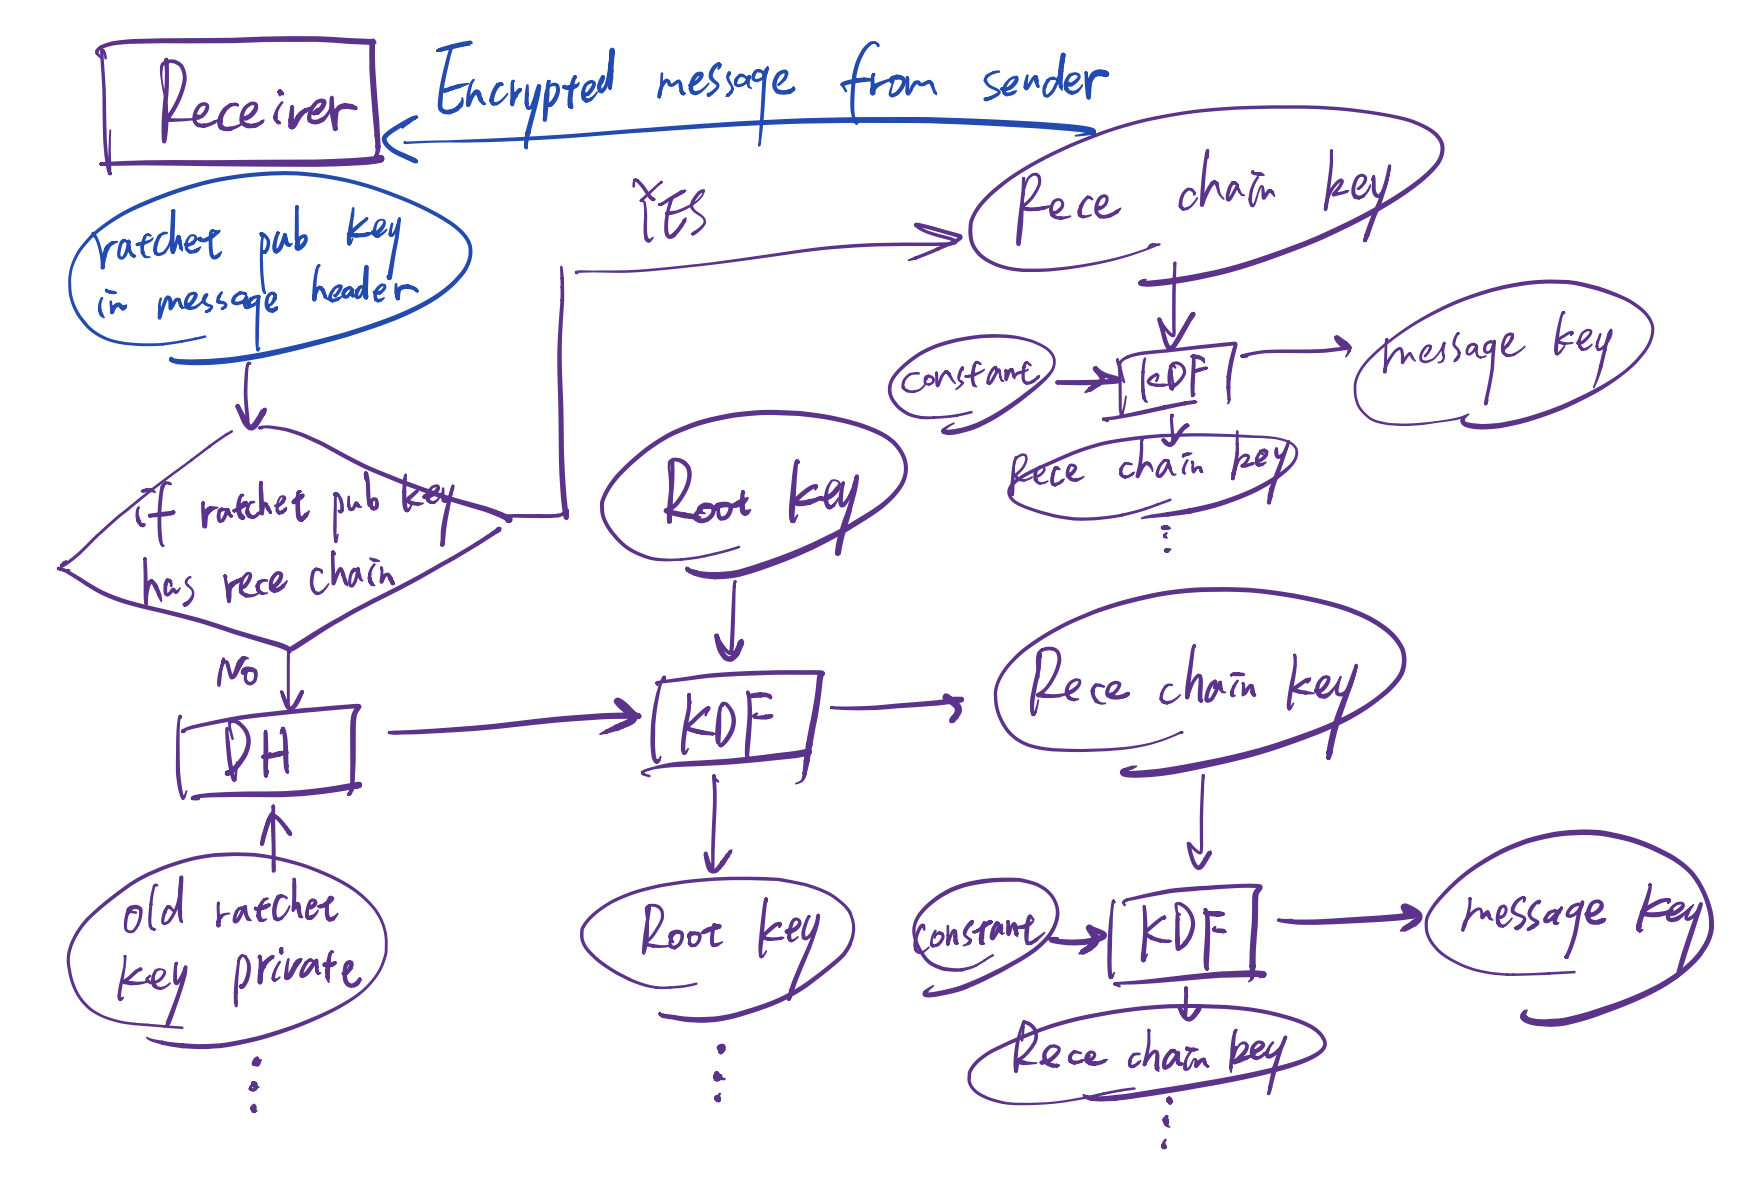
\includegraphics[scale=.5]{../3-Background/resources/DH-rece.png}\\
Figure 4.7: \textit{The testing report of junit tests in the client}
\end{center}

\begin{center}
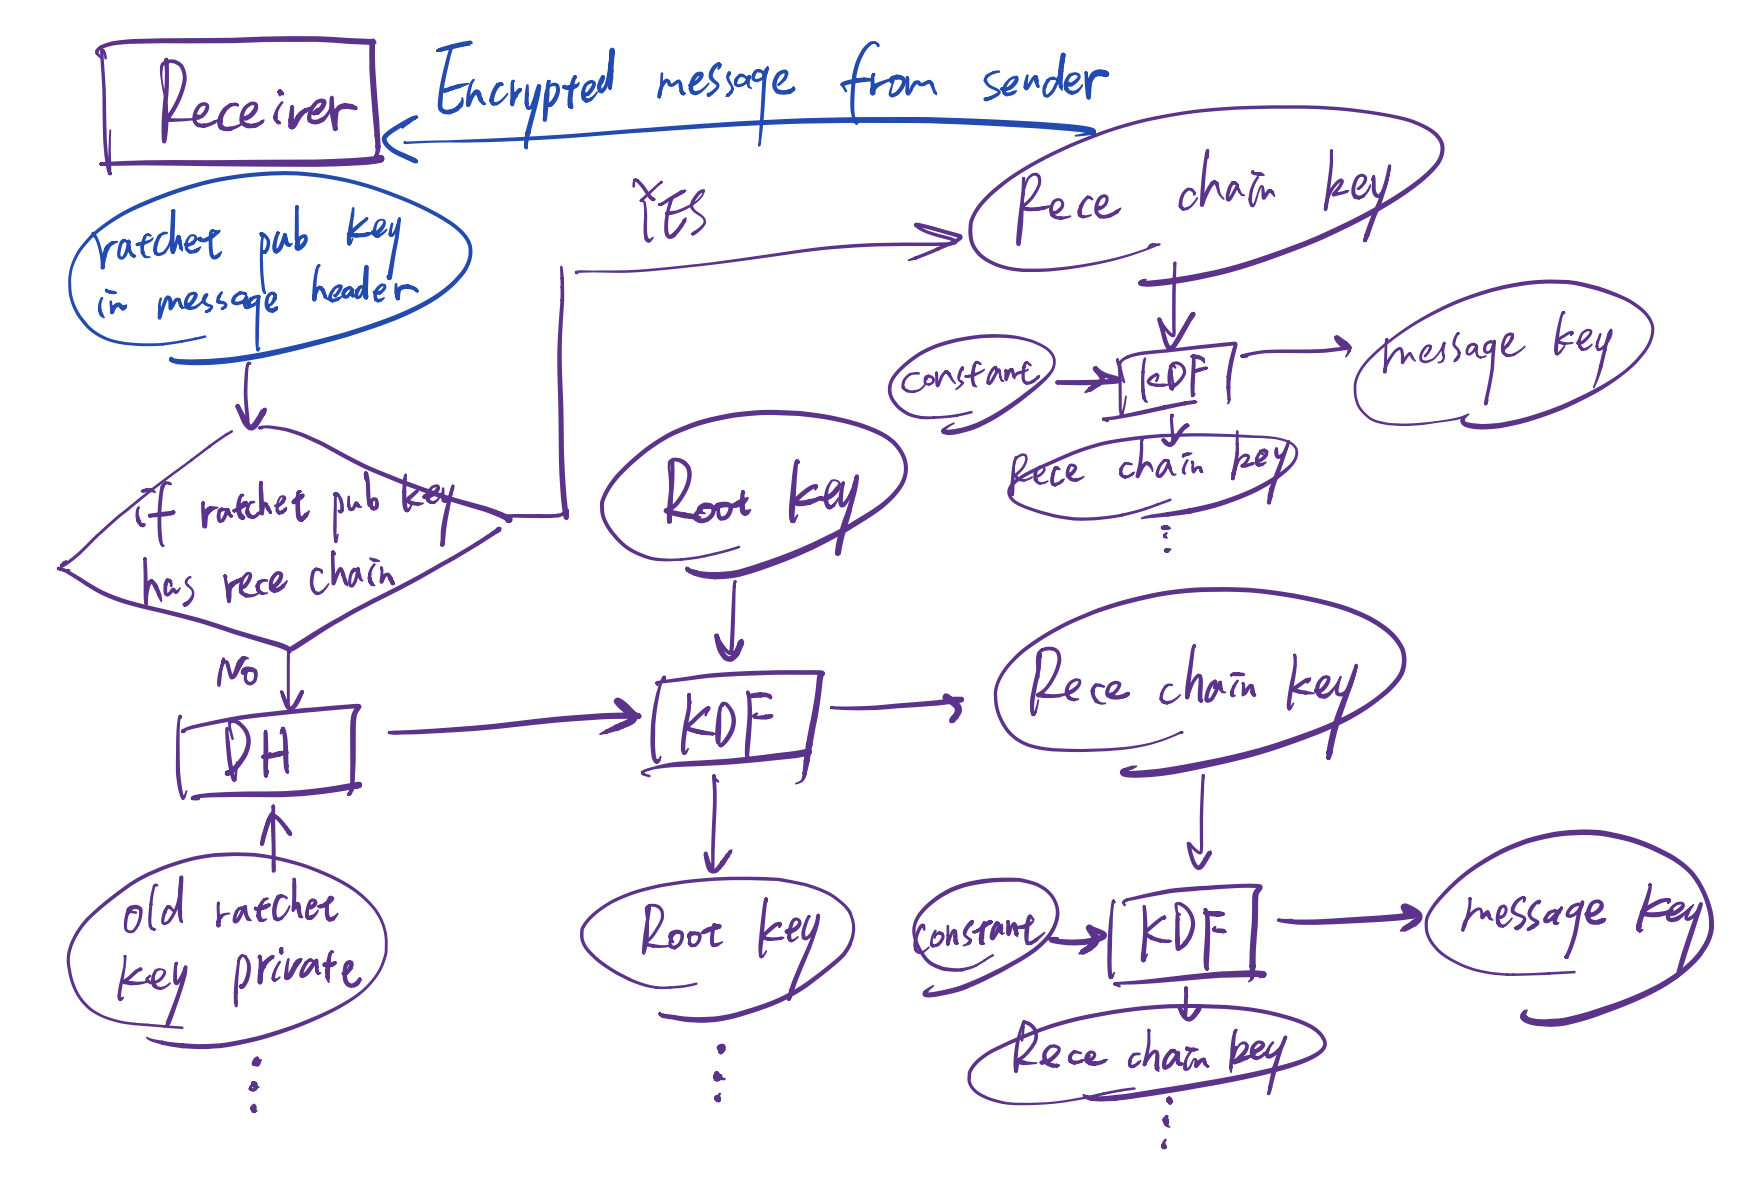
\includegraphics[scale=.5]{../3-Background/resources/DH-rece.png}\\
Figure 4.8: \textit{The testing report of junit tests in the server}
\end{center}

The black-box testing mainly tests the pairwise chat, group chat function and pairwise chat fingerprint verification. The situations includes the initialization, chatting and switching. The following parts present the result of different situations. Before all the testing, assuming there are three accounts called Alice, Bob and Cathy already been registered. The deviceId of them is 1 in default.

\begin{enumerate}[label=(\roman*)]
\item Pairwise chat testing

In the synchronous environment, Alice and Bob are both online. First Alice initializes the pairwise chat with Bob, after the shown of waiting alert, Alice could send messages to the Bob. The figure 4.9 and figure 4.10 present the initialization and chatting of pairwise chat respectively.

\begin{center}
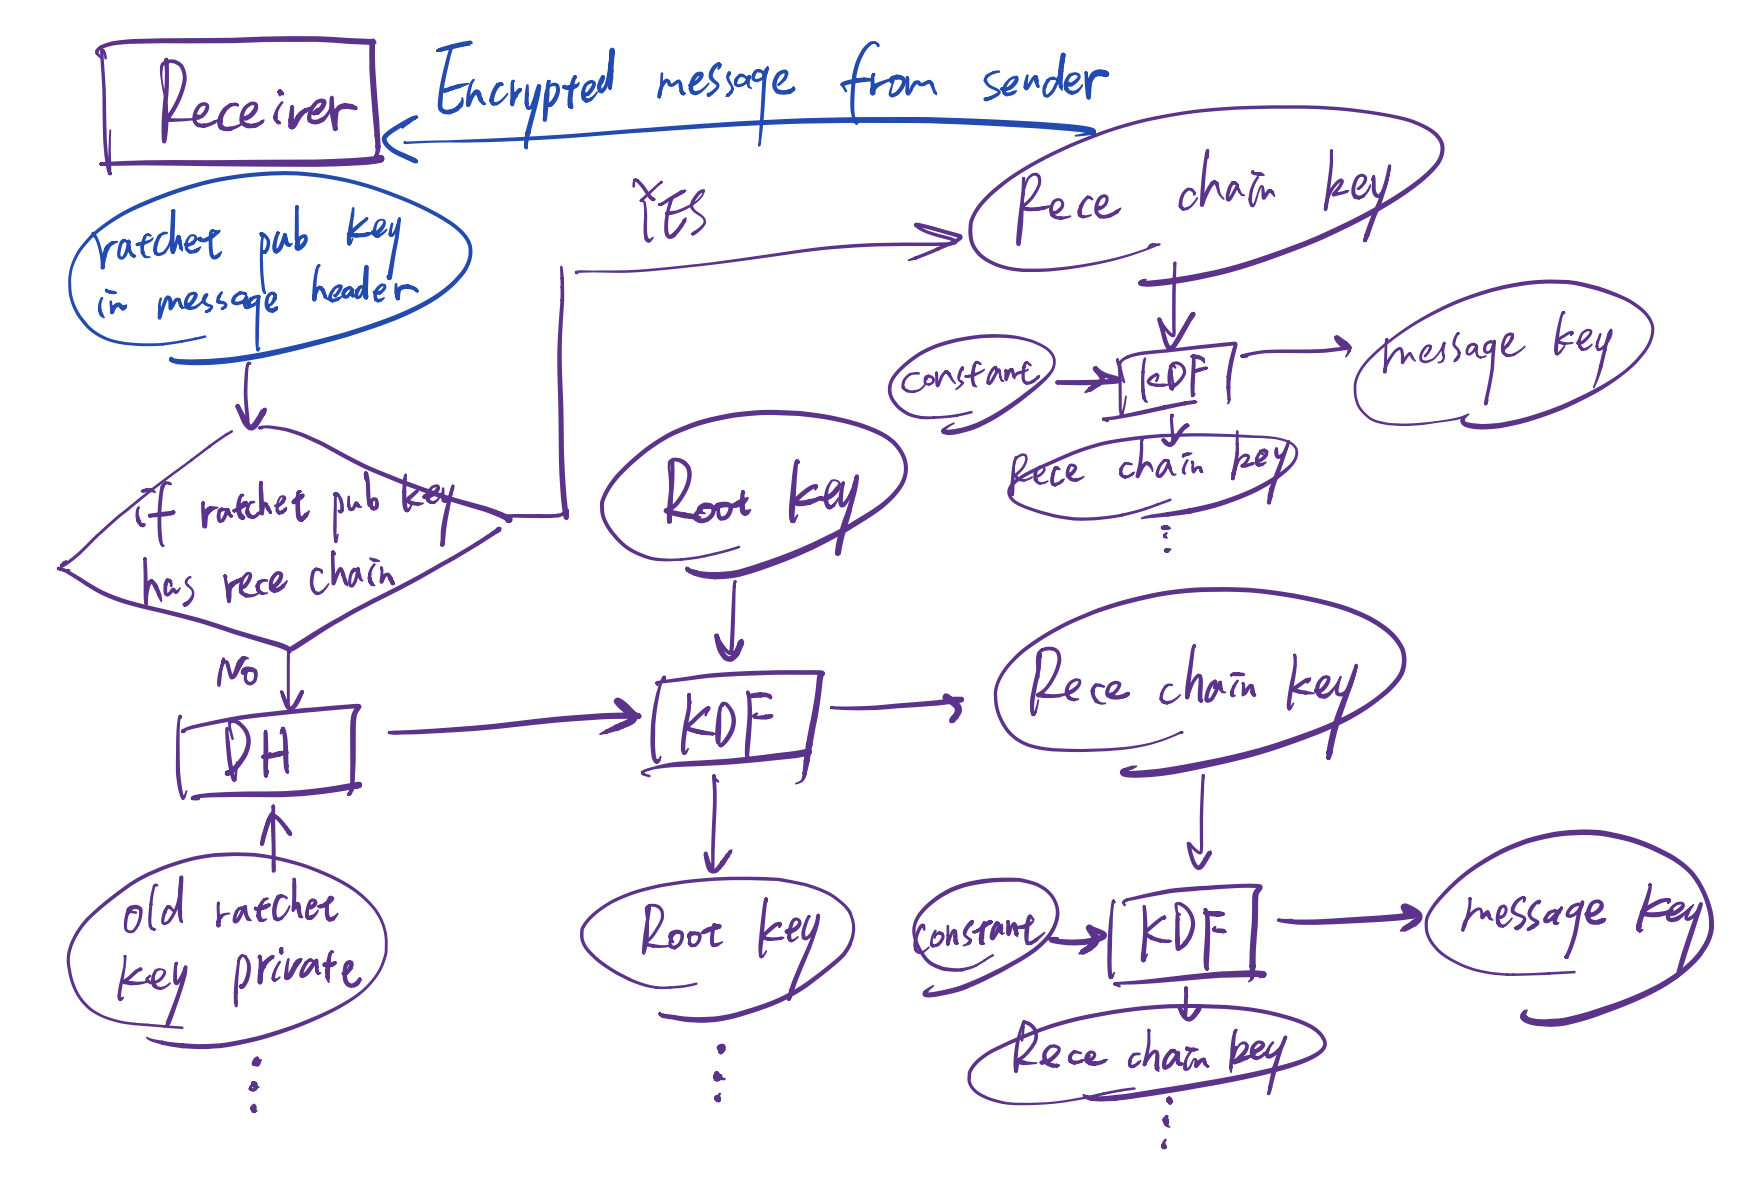
\includegraphics[scale=.5]{../3-Background/resources/DH-rece.png}\\
Figure 4.9: \textit{The initialization testing of pairwise chat}
\end{center}

\begin{center}
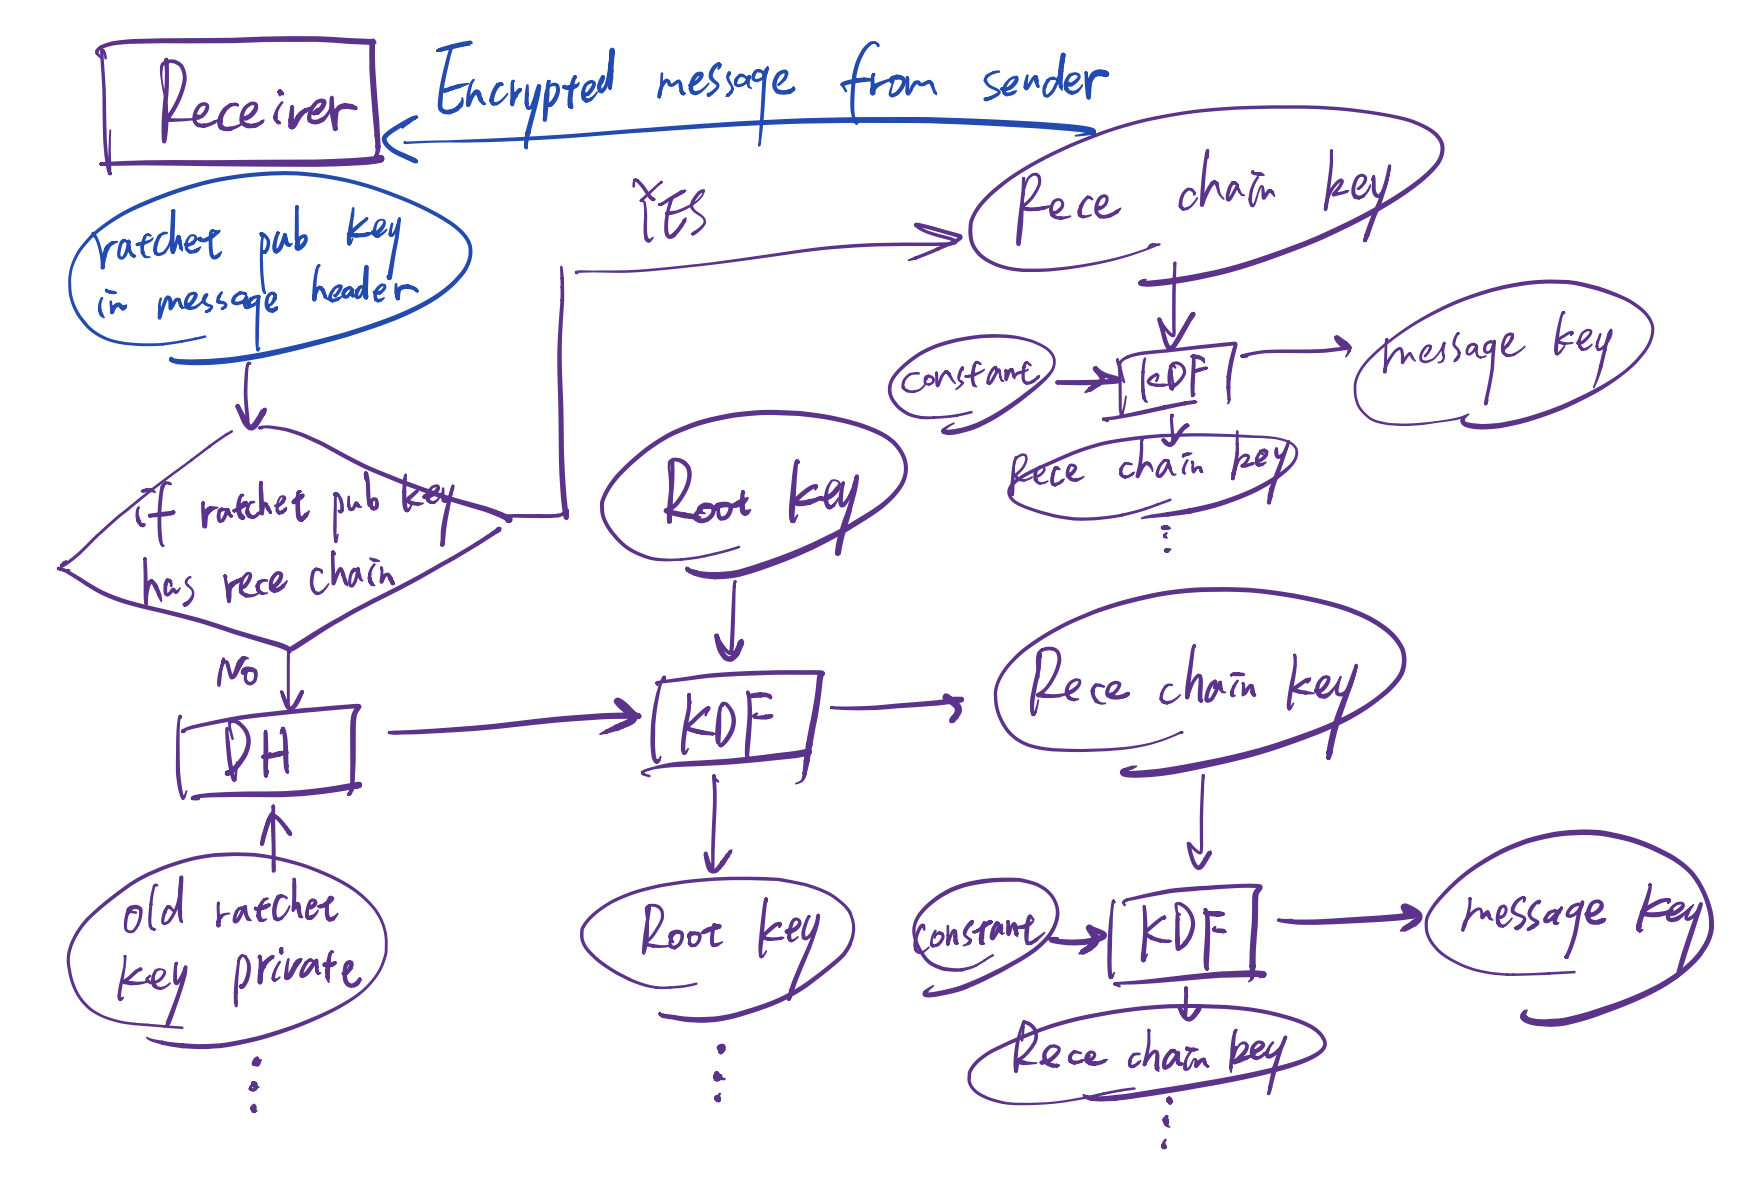
\includegraphics[scale=.5]{../3-Background/resources/DH-rece.png}\\
Figure 4.10: \textit{The chatting testing of pairwise chat}
\end{center}

In the asynchronous environment, only Alice is online while Bob is offline. Alice sends Bob some messages and see whether Bob gets the messages once login. After testing, the pairwise chat could work correctly in this situation. This testing also covers the tests of history message storage and Signal states storage.

\item Group chat testing

For the purpose of testing group chat in synchronous environment, Alice, Bob and Cathy are supposed to be online at the same time. While group chatting, the creator of the group chat Alice should request other's key bundles first for secure connection with them. Then generation and distribution of sender key is required. After the shown of waiting alert, Alice can send messages to the members. On Bob and Cathy sides, once they received the sender key from Alice, the initialization of the group chat starts in the meanwhile as Alice does. Then all the members could chat in the group. The figure 4.11 and figure 4.12 present the initialization and chatting of group chat respectively.

\begin{center}
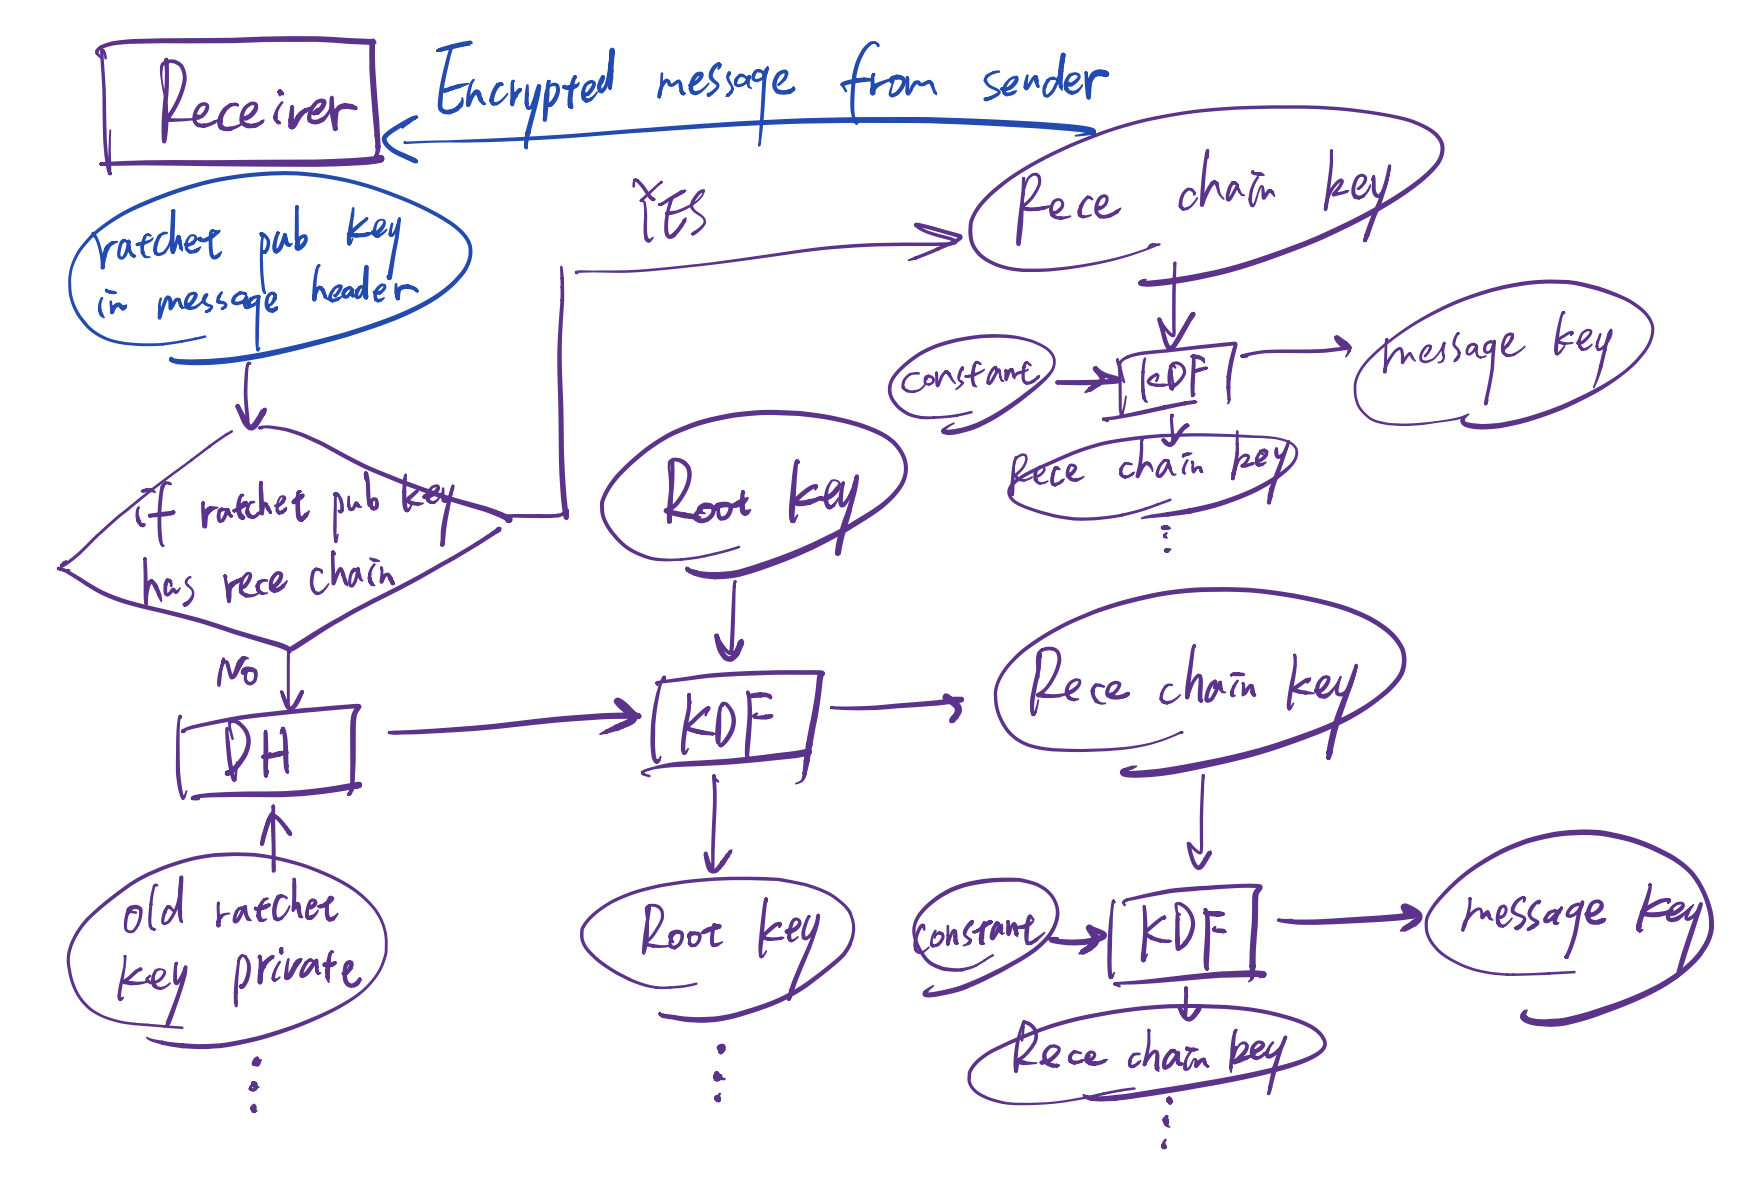
\includegraphics[scale=.5]{../3-Background/resources/DH-rece.png}\\
Figure 4.11: \textit{The initialization testing of group chat}
\end{center}

\begin{center}
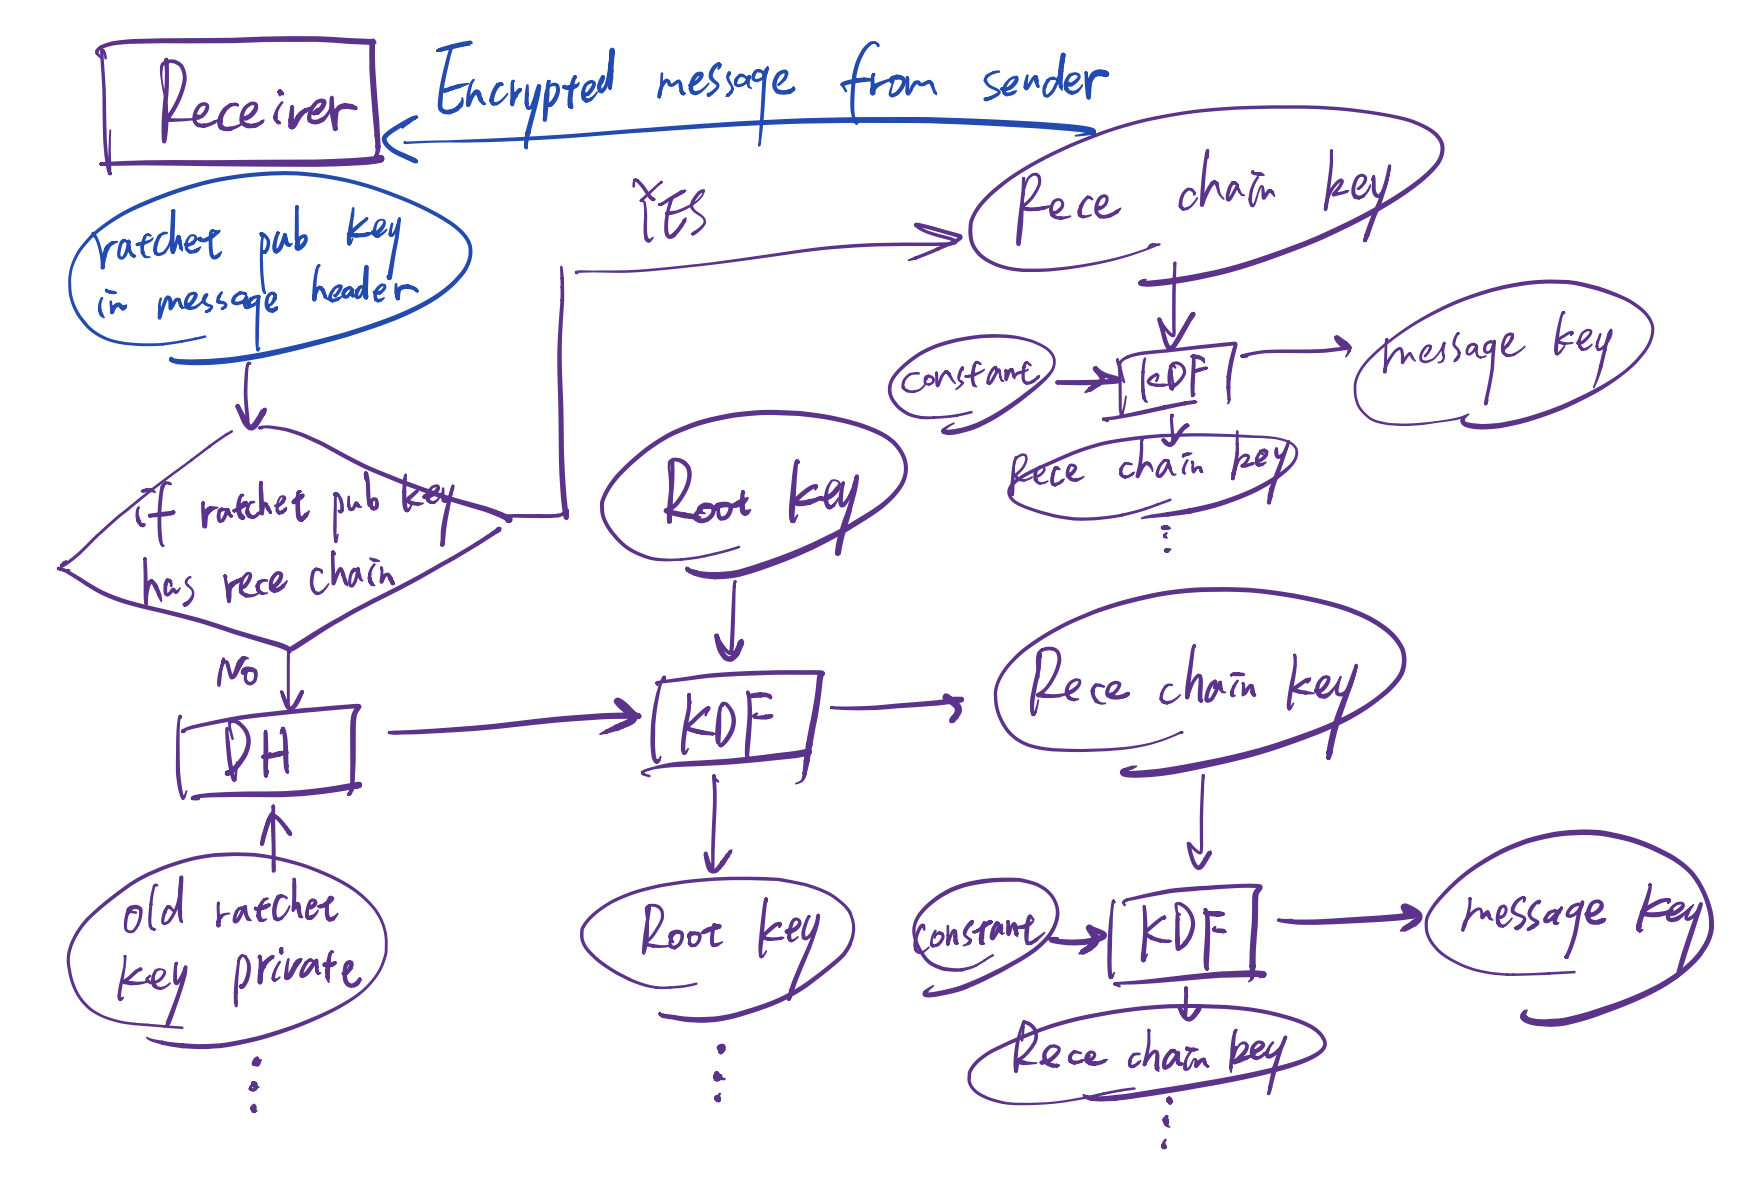
\includegraphics[scale=.5]{../3-Background/resources/DH-rece.png}\\
Figure 4.12: \textit{The chatting testing of group chat}
\end{center}

In the asynchronous environment, Cathy is required to log out first, Then Alice and Bob would have some chats during this time slot. Once Cathy login again, Cathy could receive the undeliverable messages and chat with members means the group chat could work as expected in the asynchronous environment.

\item Switch device testing

The stability of chat after switching device is essential in the multi-device system. To test if both pairwise chat and group chat could work correctly after switching devices, there is a pairwise chat and a group chat created already. Alice has a pairwise chat with Bob and a group chat with Bob and Cathy. First Bob is required to log out and register a new account with deviceId 2. After the reinitialization, both pairwise chat and group chat are supposed to work correctly including receiving and sending messages. The figure 4.13 and figure 4.14 present the reinitialization and chatting in this situation.

\begin{center}
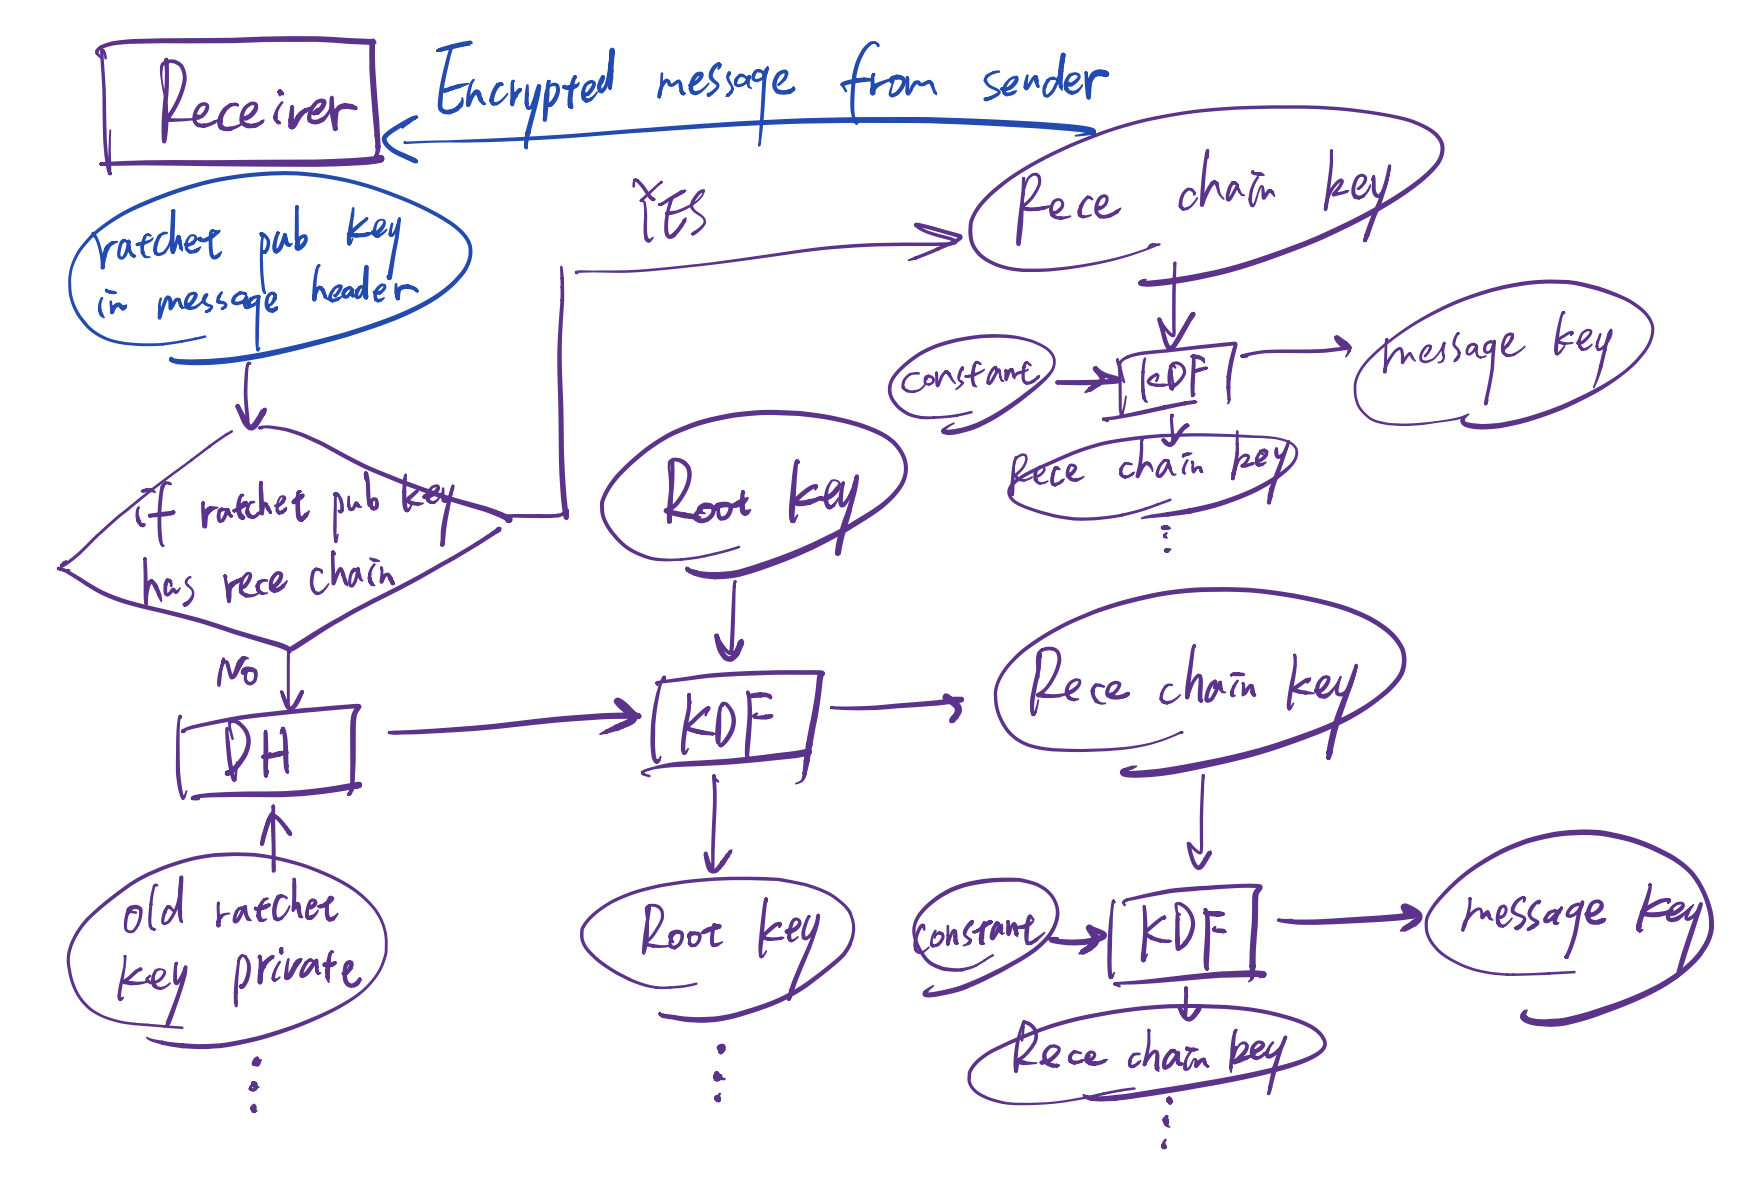
\includegraphics[scale=.5]{../3-Background/resources/DH-rece.png}\\
Figure 4.13: \textit{The reinitialization of group chat after switching the device}
\end{center}

\begin{center}
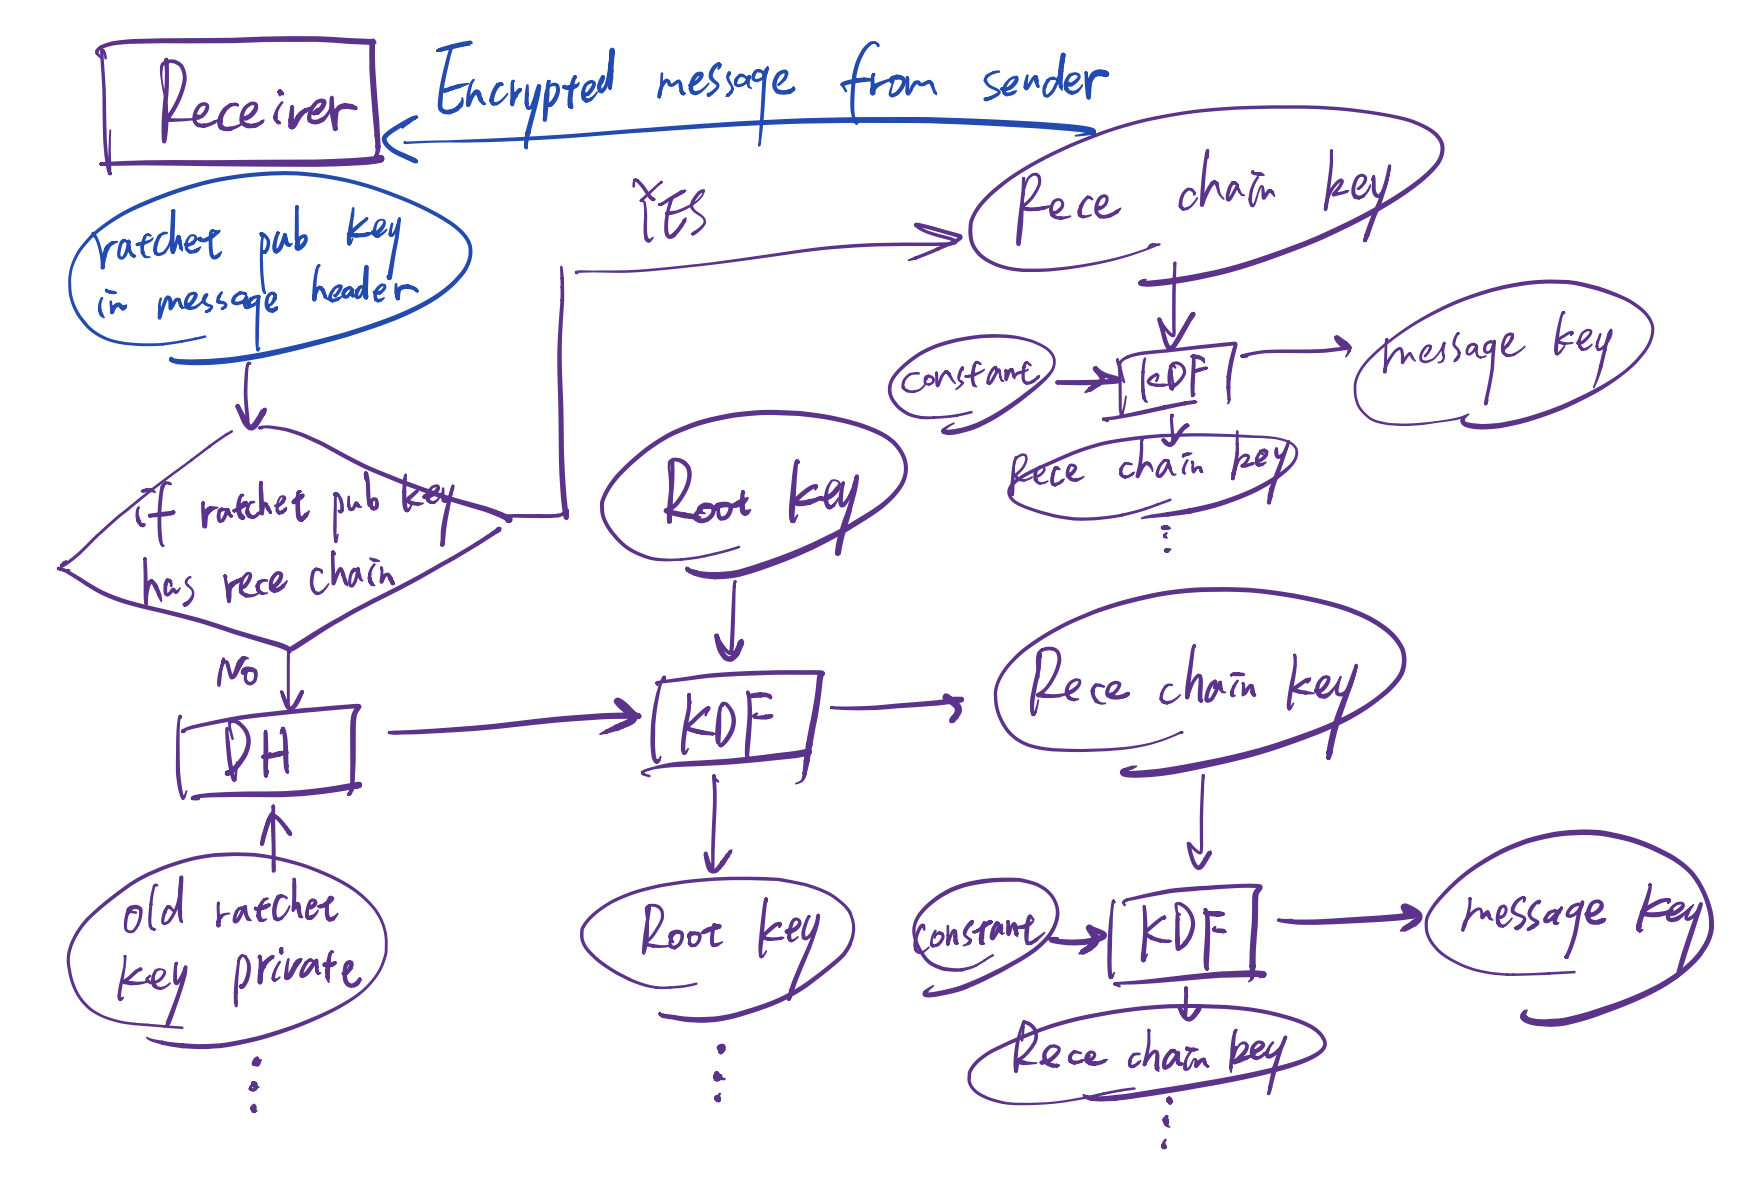
\includegraphics[scale=.5]{../3-Background/resources/DH-rece.png}\\
Figure 4.14: \textit{The chatting of group chat after switching the device}
\end{center}

\item Pairwise chat fingerprint verification

The testing pairwise chat fingerprint verification between Alice and Bob requires there is an already created pairwise chat between them. After clicking the verify button on both Alice and Bob sides, the information alert including the fingerprint of the chat is shown in the client. The figure 4.15 and figure 4.16 present the result of this function.

\begin{center}
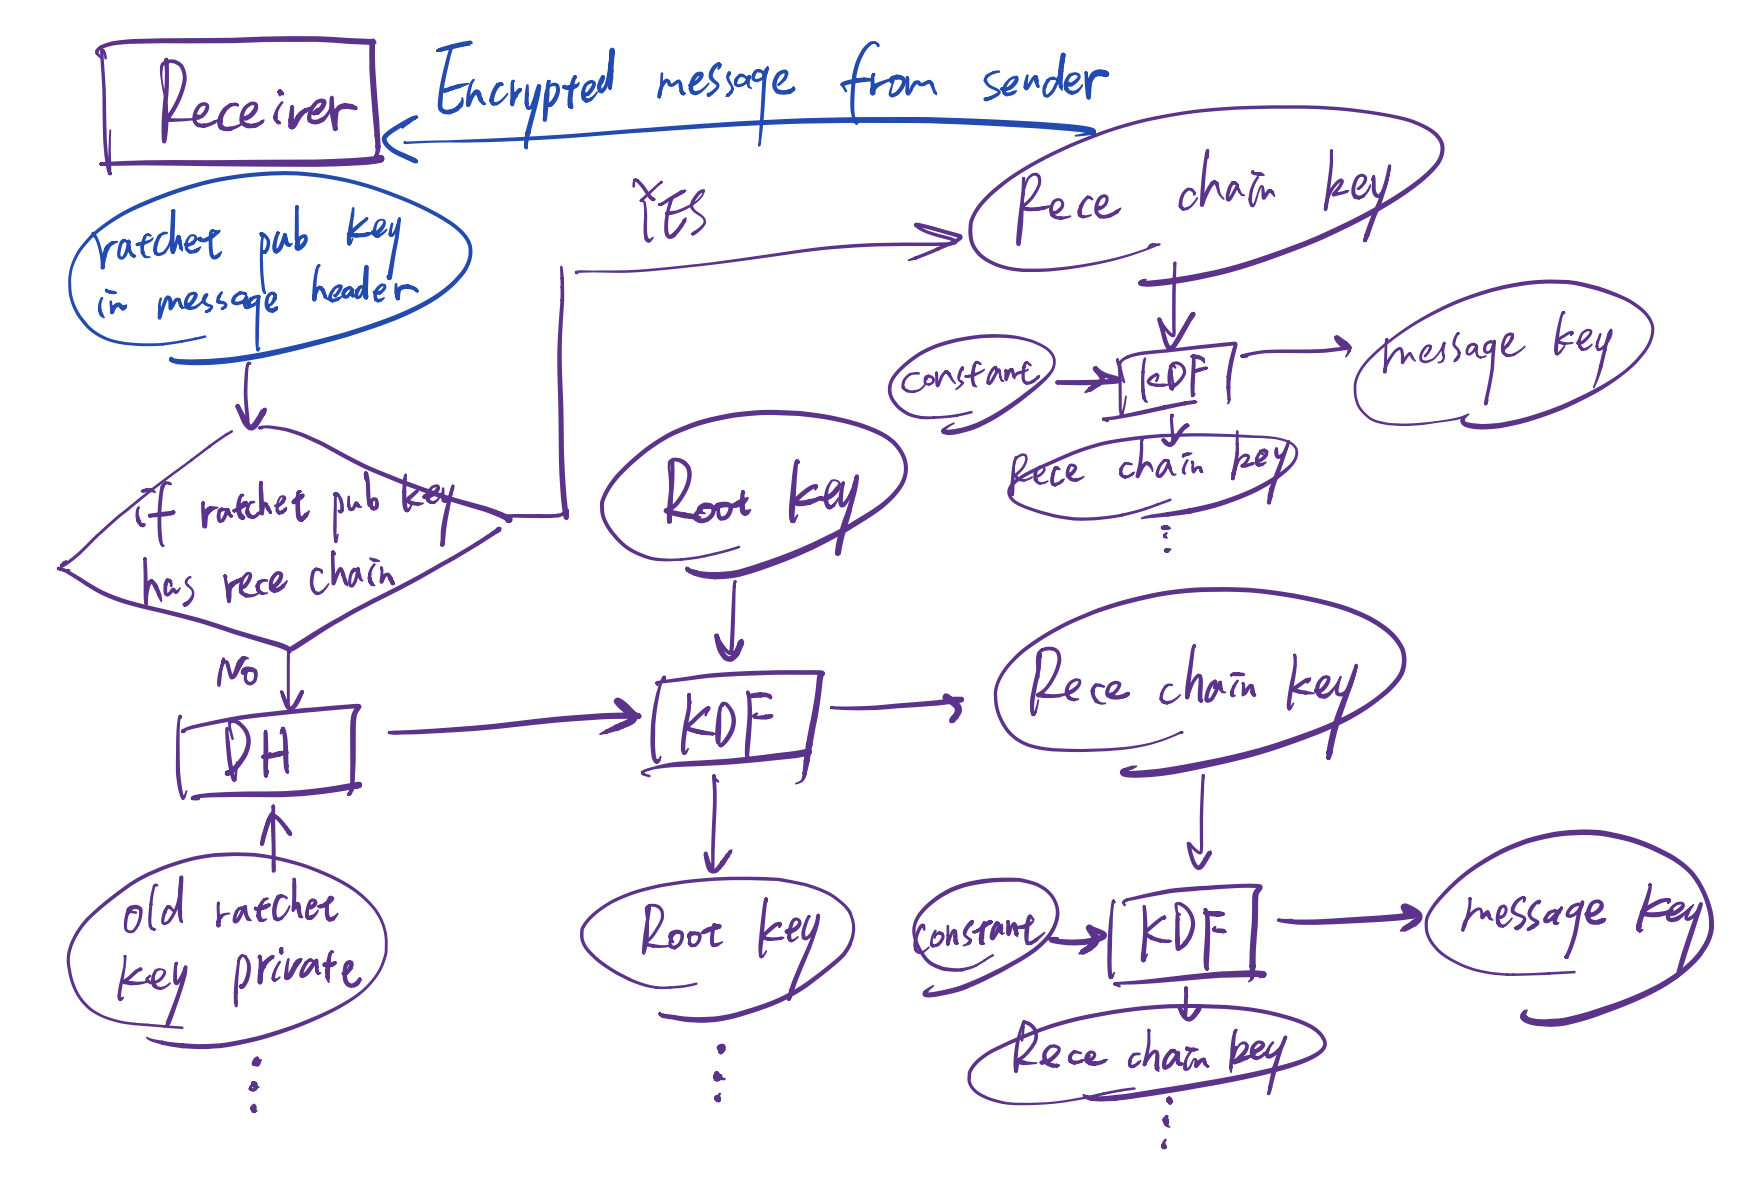
\includegraphics[scale=.5]{../3-Background/resources/DH-rece.png}\\
Figure 4.15: \textit{The fingerprint of pairwise chat on Alice side}
\end{center}

\begin{center}
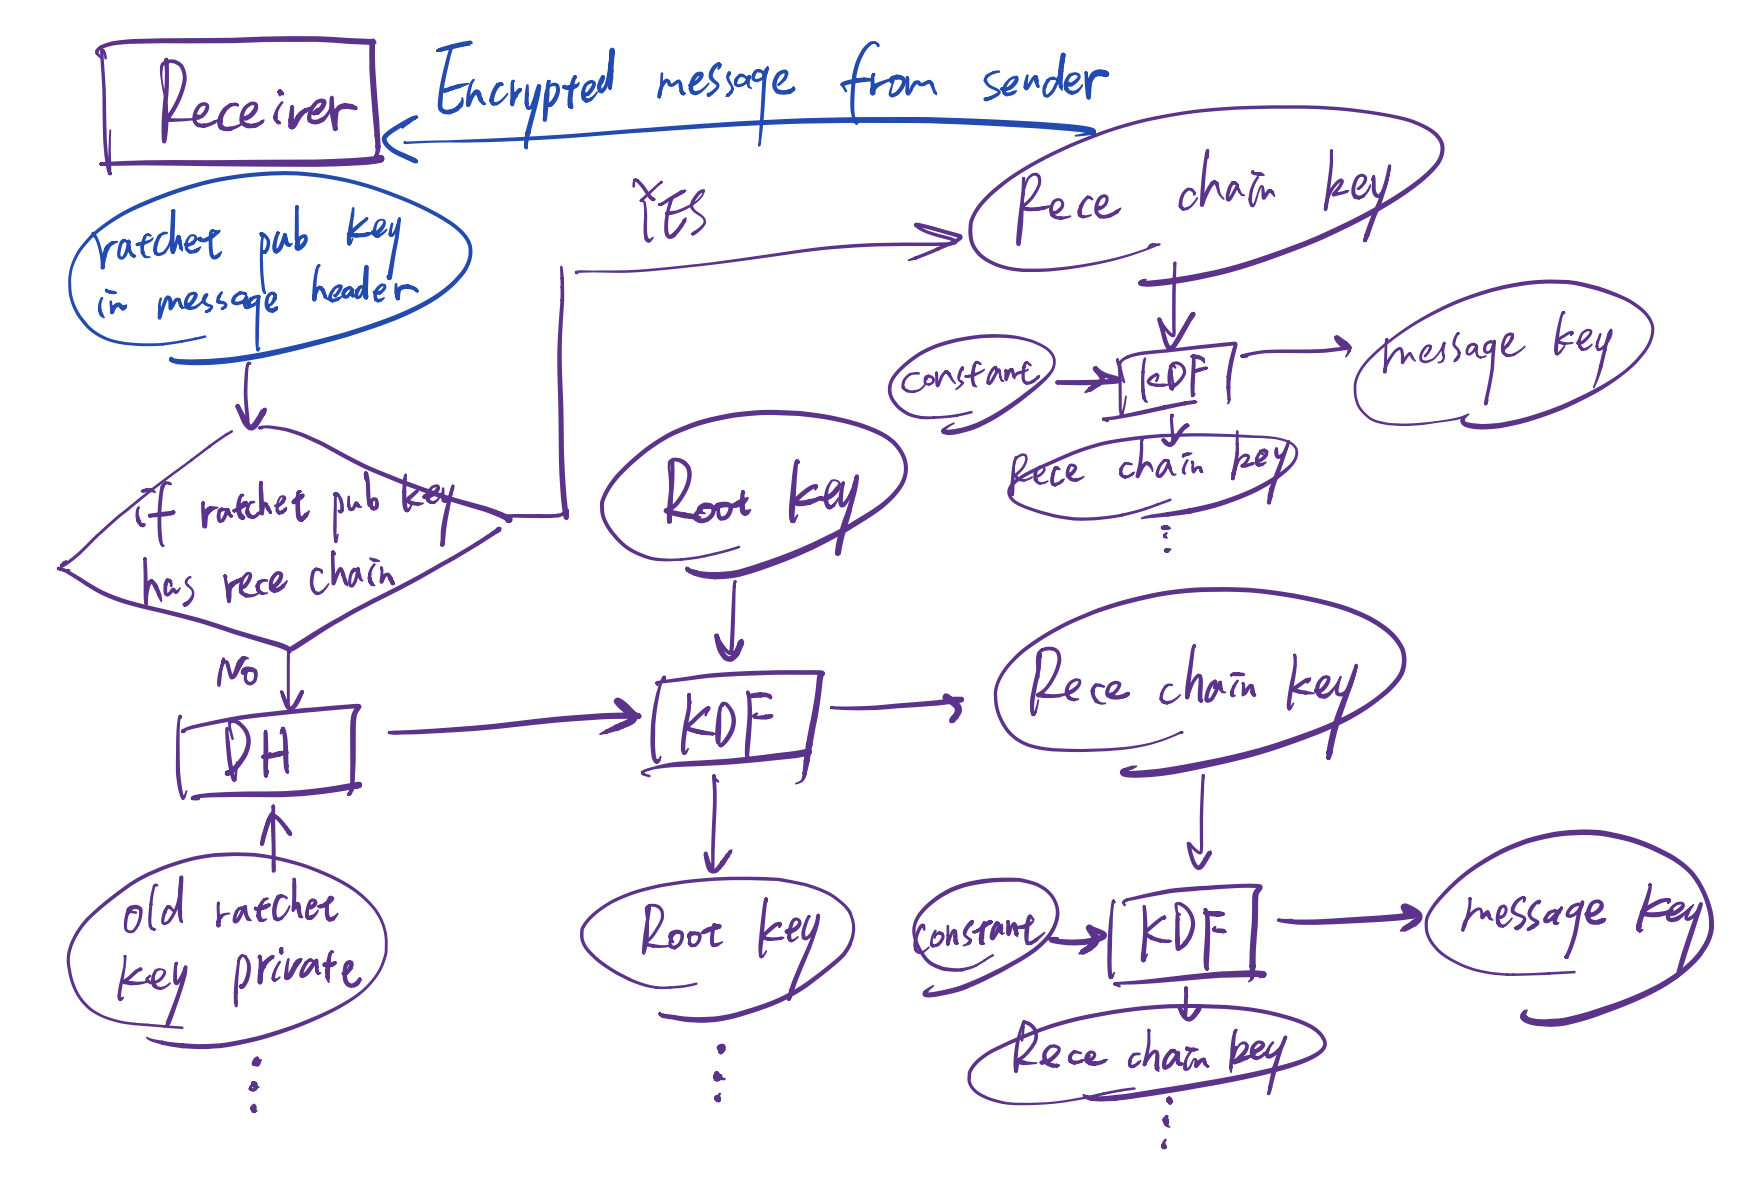
\includegraphics[scale=.5]{../3-Background/resources/DH-rece.png}\\
Figure 4.16: \textit{The fingerprint of pairwise chat on Bob side}
\end{center}

\end{enumerate}

\subsection{Project management}
The development of the project is completed within three months, so planning a proper schedule is necessary. In the first three weeks, reading lots of papers and website resources is essential to have a deep understanding about the Signal Protocol. Then determining the requirements of users and the application specification is the precondition of implementation. Once the prototype is determined, the implementation could start to develop.

During implementing, having a proper git branch structure does more with less. All the new functions are developed in branch ZiyanWang, after the implementation and testing, the code would be merged to the master branch. This process could make sure the new added functions would not break down the whole system while developing. Sometimes finding the unexpected bug is usual during development, the tests could not cover all the aspects. When fixing the issues, the developing code could be stashed for not confusing the thinking.

Commit records of git is also useful during developing. Make sure every steps is small. For example, every new added function and every fixing of issues could be committed as a new record. That would make the code version clearer, once the system breaks down the project could roll back to the latest version without too much loss.

\subsection{Results and evaluation}
After all the implementation of new functions in the whole system, the chat system is upgraded to a secure E2EE chat system. The features of it include the pairwise chat, group chat, switching device and messages backup etc. Users could communicate with each other in secure based on Signal Protocol. To verify the Signal Protocol works correctly in this system, the message key obtained from the symmetric ratchet is printed in client after each encryption and decryption. Comparing two message keys of two parties is a clear proof of the implementation of Signal Protocol. The figure 4.17 and figure 4.18 present the printed message keys of one pairwise chat's two parties respectively.

\begin{center}
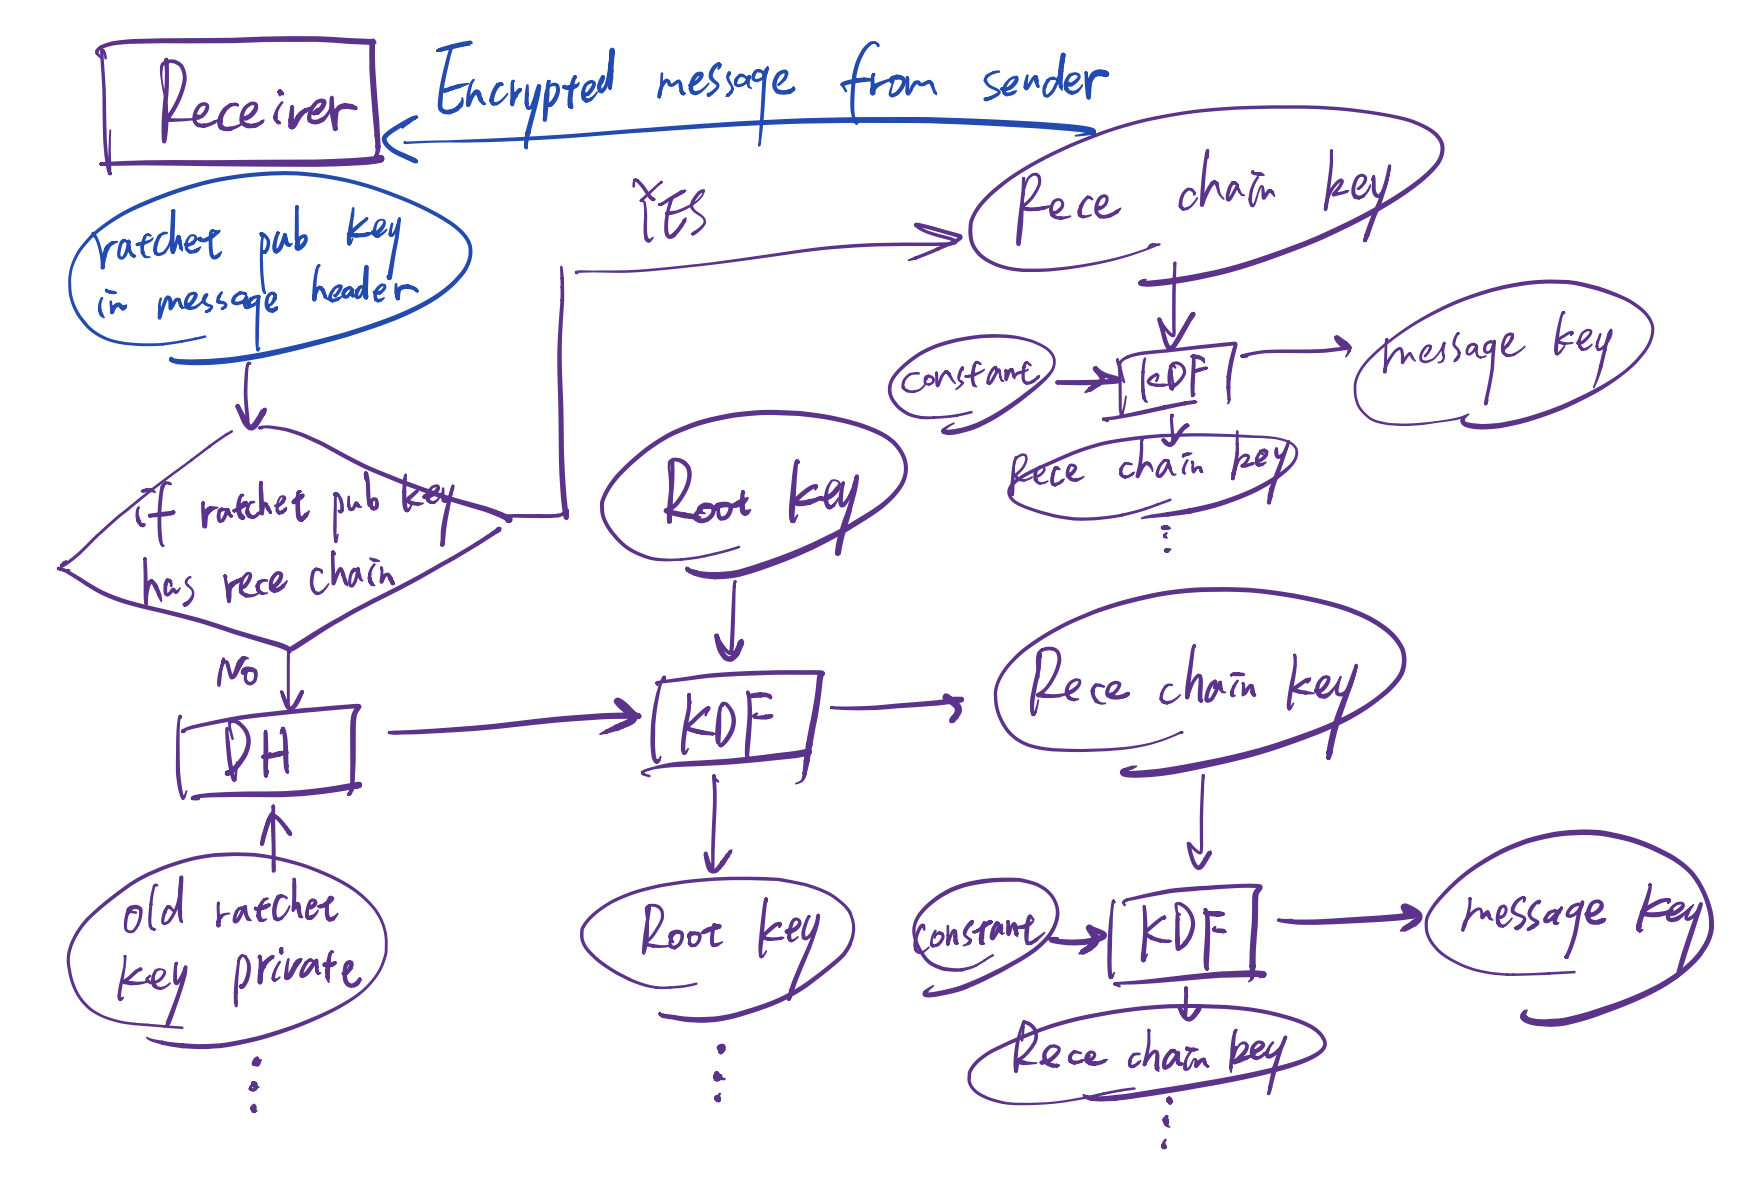
\includegraphics[scale=.5]{../3-Background/resources/DH-rece.png}\\
Figure 4.17: \textit{The message key after encryption on sender side}
\end{center}

\begin{center}
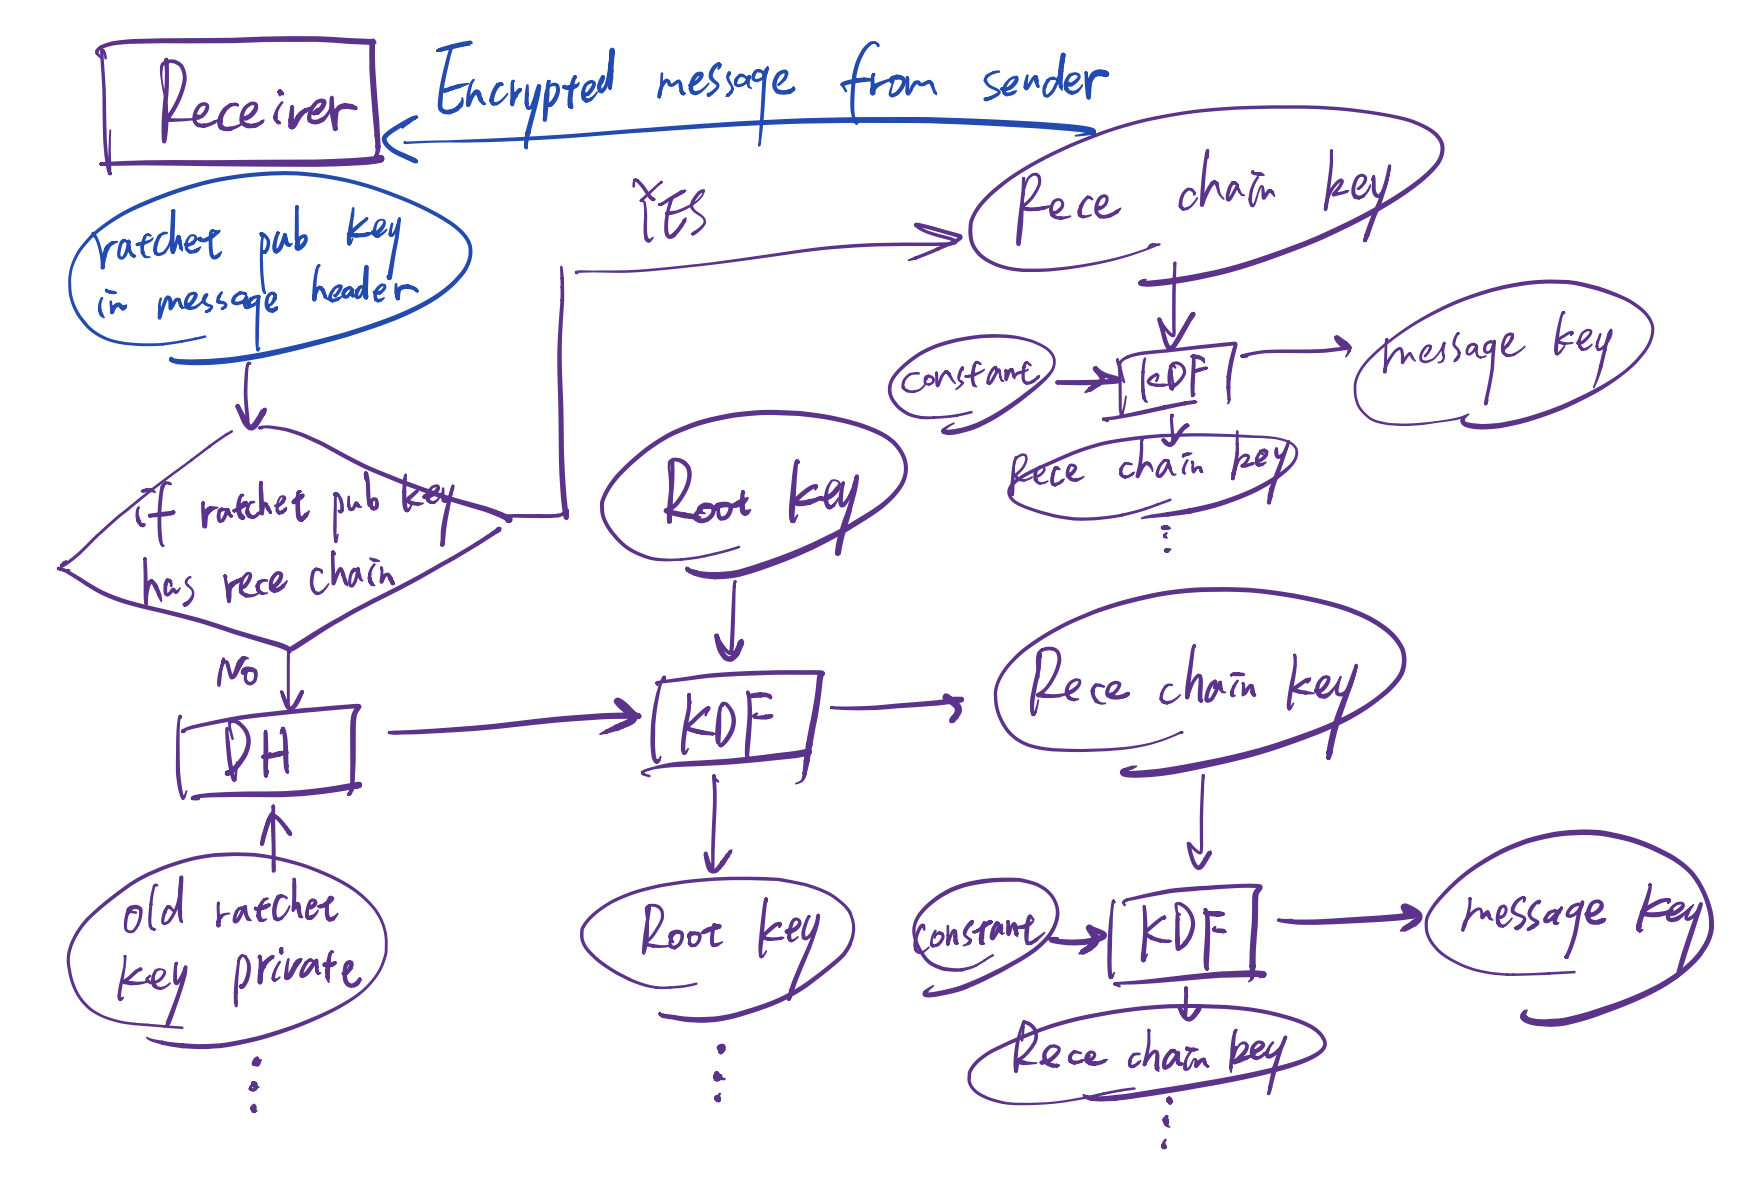
\includegraphics[scale=.5]{../3-Background/resources/DH-rece.png}\\
Figure 4.18: \textit{The message key after decryption on receiver side}
\end{center}

The final product basically accords with the initial design in terms of functions. After all implementation completed, the system could work correctly in pairwise chat, group chat and multi-device system etc.

There are still several defects that influence the robustness and performance of the system. For example, the system does not implement the SQL injection attack prevention system. The adversary could use the SQL inquiry flaw to get the user privacy. Also due to the IO structure of the previous system, the switching device function may not work as expected after a few times of continuous switches. As for the performance, the server verification user function inquires the data from database several times which causes the time performance issue. And since the thread pool is not used to handle the multi threads work allocation, the server may break down when the great amount of users login in together. Besides, because the server uses the SSH to connect to the database served by bham, the connection may be broken in a poor network environment which would cause the whole system down.

\clearpage
\section{Discussion}

\subsection{Achievements}
The achievements of the project could be discussed on several aspects including function realization and the system stability.

After the main function realization completed, the features of the upgraded system could be listed as following:

\begin{itemize}
\item Login and register validation via jdbc
\item Secure the content within pairwise chat and group chat
\item Save encrypted signal storages and history messages at client local
\item Multi-device system
\item Message backup between devices
\item Work in both asynchronous and synchronous environment.
\item Fingerprint verification for pairwise chat.
\end{itemize}

In consideration of the system stability, the project uses junit testing and black-box testing. The junit testing covers almost all the logic functions that could be tested and all the junit tests have been passed. In black-box testing, different testing situations are considered. The issues discovered during the testing have been fixed at the end.

As a security project, the secure E2EE chat system achieves the goal of implementing Signal Protocol. After testing, the system could work as expected to secure the content during communication. The users' privacy within the system have been guaranteed basically. However, as a commercial product, the security of the whole system still needs to be improved like preventing SQL injection attack.

\subsection{Defects}
The final product of the project could not compete with the existed related commercial product due to the defects. The defects would be introduced with two parts including the client and server.

\begin{enumerate}[label=(\roman*)]
\item Defects in the client

In the Signal related aspect, the user could not verify the security of the group chat via fingerprint. The fingerprint of the pairwise chat could be generated and compared to check whether the session is monitored by adversary. The users could only perceive something wrong in group chat when the related pairwise chat has the failed verification. The break-in recovery feature is also not implemented in the client. In Signal system, the signed pre key is a mid-term key of a user. The signed pre key is required to be updated within several weeks for security consideration. Also the function that appends the users' pre keys is not implemented in the client. Although these functions are not essential for a secure E2EE chat system, but the missing of them could make the whole system vulnerable.

In the structure aspect, due to the existing project structure like IO structure, the system may occur unexpected errors sometimes. For example, when a user switches devices several times continuously, the group chat would not be reinitialized correctly. Since this project belongs to a security project, refactoring is not the own job during developing. But the issues caused by the project structure decreases the robustness of the whole system.

\item Defects in the server

In the Signal related aspect, the server does not implement the function that requesting new pre keys once the users' pre keys are used out. Although it does not influence the system working correctly, this would reduce the security of X3DH algorithm. Besides, the management of group chat is supposed to be enriched including adding or removing members.

In the project structure aspect, the persistence of undeliverable messages are not implemented. The server does not store them in database, once the server is rebooted, all the undeliverable messages would be lost. This defect would influence the system working incorrectly in asynchronous environment. As a secure chat system, it's a regret that the sever does not prevent other type's attacks such as SQL injection attack and DDoS attack.

In consideration of the performance, the login and registration verification in the server are also required to be optimized. The SQL execution times during the login verification is too much so that causing a large amount of time loss in the poor network environment. Besides due to the limited time and the multi threads structure, the sever may break down if numerous users login in the meanwhile.

\end{enumerate}

\subsection{Evolution}
Corresponding to the defects of the system, the evolution could be discussed on the client and server side too.

\begin{enumerate}[label=(\roman*)]
\item Evolution in the client

The fingerprint verification function of group chat could be implemented by using members' identity keys. The fingerprint of the group chat would be generated by combining all the members' identity key and members could compare it with each other to make sure the group chat is not monitored.

To achieve the break-in recovery feature, the users should be allowed to update their identity key and signed pre key. Once the user updated key bundle, all the other users would be informed and reinitialize the related chat immediately.

In the future development, the system could refactor the client structure including IO structure and connectionData format. Refactoring IO structure allows the client could handle the asynchronous functions more easier. The unexpected issues would decrease after the refactoring. The transmission data's format is also supposed to be refactored, all the payload could be serialized to bytes for decreasing the number of types in connectionData. Besides, it's better to refactor the transmission protocol to make the client could communicate with other Signal compatible sever. This could proof the Signal Protocol is implemented and working correctly inside the system.

\item Evolution in the sever

To improve the X3DH security, the sever is supposed to request new pre keys from users once the pre keys are used out. In the current system, the sever would return a null value back if there is no pre key related to the user.

As for the management of group chat, the sever does not verify if the sender is one of the members when the user doing some group operations. For example, if the user is out of the group, the user should not be allowed to ask all the other members to update the sender key. This alteration could provide the stability of group chat function.

While verify the user identifier during login and registration, the sever could combine several SQL executions together to reduce the time loss. Another solution of this performance problem is loading all the users information once the sever boots, then verifying user identifier in cache is faster then inquiry from database. But in this solution, the space would cost a lot if there are a large mount of registered users.

\end{enumerate}

\clearpage
\section{Conclusion}

\subsection{summary}
This project is aim to implement a secure E2EE chat system based on Signal Protocol. The final artifact achieves the goal set at the beginning. The previous product is a traditional chat system that both the client and the server could access the content of communication. Although TLS is used to secure the transmission package, some security features such as the forward security and future security are missing in the previous system. Once the one of the encrypted packages is cracked, all the privacy information would be leaked during the communication. Besides, the security of the sever is essential in previous system: once the server is attacked, all the privacy information like history messages would be accessed by adversary. In the secure E2EE chat system, the server is just responsible for storing users' key bundles and basic information. The loss would not be inestimable when the server is down.

The final product implements the E2EE feature in the system. Users could have pairwise chat and group chat secretly. The system not only develops the functions that secure the communication content between users, but also implements other reliable functions such as multi-device system, message backup and pairwise chat verification. The upgraded chat system could satisfy almost all the requirements of users in security aspect. However, the defects of the system like not appending pre keys and unexpected issues after continuous device switching influence the robustness and performance. Generally, the final artifact of this project achieves the goals that set at the beginning and solve the problem that could not satisfy users' security requirements previously.

\subsection{evaluation}
In general, the solution that using the Signal Protocol to improve the security of the chat system satisfy the users' security requirements. There are several advantages and disadvantages of the final product could be evaluated. The evaluation could be discussed in aspects including functionality, security and stability.

In functionality aspect, the core parts of the Signal related codes are invoked from the libsignal-protocol-java lib. After having a deep understanding about the Signal Protocol and reading the source code in detail, the Signal related functions are implemented properly. The users could chat with others in pairwise and group chat way as before. The upgraded system does not effect the functionality basically. The only alteration is that the server does not maintain the history messages. The user is required to save the Signal related storages and chat data.

In security aspect, all the security features including forward security, future security and the deniability are implemented inside the Signal Protocol. Since the Signal Protocol is implemented in the system properly, the security of users' communication content is guaranteed. But the system does not consider other type of attacks. The users privacy could be accessed via SQL injection attack and the chat data would be leaked once the encrypted storages are cracked in the client. So the transmission security of users is improved but the security of the whole system still needs evolution.

In stability aspect, the user could have continuous using experience because of the Signal storages and chat data storages. The system could work in both asynchronous and synchronous environments. Users could switch devices back and forward without message lost. The whole system works as expected in the case of a small number of users. But due to the previous structure of the project, the system may occur some issues in the case of a large number of users or in the case of continuous device switching. So the stability of the system is the weakest part, the final artifact is not suggested for business use. 

\clearpage

\lhead{}\chead{MSc. Project Report :: \nouppercase{\leftmark}}\rhead{}
\phantomsection
\addcontentsline{toc}{section}{References}
\bibliographystyle{bhamthesis} 
\bibliography{bib_file}

\clearpage

\section{Appendices}
The git repository address of this project is \href{https://git-teaching.cs.bham.ac.uk/mod-msc-proj-2019/zxw989}{https://git-teaching.cs.bham.ac.uk/mod-msc-proj-2019/zxw989}
\subsection{Project structure of git repository}
The structure of the git repository could be divided into two parts including socotra-client and socotra-server.

Both the client and the server project use gradle to manage. The logic code and testing code are contained in the /src/main and the /src/test directory respectively. Inside the /src/main directory, the functional part is developed in /java directory. The resources directory maintains the static files including the view files and property files for project config.

The main entry of the program in the server is the Server.java file. The core functions in the /java directory on the server side is developed inside several packages including common, jdbc and service. The common package are responsible for maintaining the common class both on client and server. The version of the common classes must be the same while development. The classes of jdbc package are used to handle the jdbc related operations. In the service package, there are classes for processing the communication with the clients.

The main entry of the program in the client is the Client.java file. The common package's duty is the same as it in the server. Since the architecture of the client project is MVC, the controller package holds the functions that control the view's changing operations and the model packages maintains the data model of the view. The implemented Signal related functions are developed in protocol package including Signal stores, encryption handler and file handler.

\subsection{Quick start of the code}
\subsubsection{Build and run}
To make the whole system work properly, the server project is required to run first. Before running the server project, it is essential to add a jdbc.properties file which includes the ssh connection information and database information in src/main/resources like:

\begin{lstlisting}
sshUser=bhamUsername
sshPassword=bhamPassword
dbUser=username
dbPassword=password
\end{lstlisting}

Because the database is severed by bham, for connecting to the bham's database service successfully, the server project is required to use SSH connection. The SSH information including sshUser and sshPassword which are them same as bham's identifier information.

The two projects both use gradle-wrapper, developers could just open either of them in intellij or eclipse simply, and use the gradle tool inside the IDE to build and run the project.

The project could be simply run without the installing the gradle, just run the following commands under the project root folder like /socotra-server or /socotra-client:

\begin{lstlisting}
./gradlew build
\end{lstlisting}

then to run the application:

\begin{lstlisting}
./gradlew run
\end{lstlisting}

Or using the gradle GUI tool inside the IDE (for intellij it's on the right side bar) is more convenience to run the corresponding tasks.

\subsubsection{Junit test}

Both two projects use junit5 to write some tests exclude socket and GUI tests. To run the test, use the gradle tool test in menu Tasks/verification or use the command in the terminal:

\begin{lstlisting}
./gradlew test
\end{lstlisting}

The test report will automatically generated by gradle in directory build/reports/tests/test/index.html.

\subsubsection{Archive and release}

For server project, you can release the .jar file, you can archive the server project as:

\begin{lstlisting}
./gradlew uploadArchives
\end{lstlisting}

then the repos foler will be generated with serveral .jar files.
For client project, it use javafx11 to build the GUI, so once you use the gradle to generate a .jar file, you need to download javafx11 sdk first, and run it as following:

\begin{lstlisting}
java --module-path $PATHTOJAVAFXSDK11 --add-modules javafx.controls,javafx.fxml,javafx.base -jar $YOURCLIENT.jar
\end{lstlisting}

\clearpage

\clearpage

\end{document}